\documentclass[conference]{IEEEtran}

\usepackage[utf8]{inputenc}
\usepackage[T1]{fontenc}
\usepackage[brazil]{babel}
\usepackage{graphicx}
\usepackage{booktabs}
\usepackage{multirow}
\usepackage{amsmath, amssymb}
\usepackage{float}
\usepackage{xcolor}
\usepackage{fancybox}
\usepackage[section]{placeins}

\graphicspath{{../assets/elections/plots/}{../assets/elections/tables/}}

\newcommand{\tablePlaceholder}[1]{%
  \begin{center}
    \fbox{\parbox{0.85\columnwidth}{%
      \centering\vspace{0.4cm}
      \textbf{[PLACEHOLDER]} \\[0.2cm]
      \textit{#1} \\[0.4cm]
    }}
  \end{center}
}

\title{Análise Estatística Descritiva do Dataset de Eleições Brasileiras de 2014:\\
Gastos de Campanha, Votos e Desigualdades Regionais entre Candidatos a Deputado Federal}

\author{
  \IEEEauthorblockN{Heitor Teixeira - 2651254}
  \IEEEauthorblockA{
    \textit{MBA: Ciência de Dados}\\
    UNIFOR\\
    Fortaleza, Brasil\\
    heitor.mba.unifor@gmail.com
  }
}

\begin{document}

\maketitle

\begin{abstract}
Este artigo apresenta uma análise estatística descritiva do dataset de
 eleições brasileiras de 2014 (D2), com foco na relação entre recursos
financeiros de campanha e desempenho eleitoral de candidatos a Deputado
Federal. O arquivo original contém 6.353 candidaturas, das quais 5.323
registraram gasto positivo e foram mantidas nas análises centrais sobre
financiamento. Além das exigências do briefing da disciplina, o trabalho
enriquece o dataset com bases públicas do TSE, adicionando informações de
partido, gênero, raça, situação eleitoral e fornecedores. O relatório cobre
os histogramas de votos e gasto para três UFs escolhidas pelo autor
(RJ, GO e AM), os respectivos gráficos de dispersão com correlação de
Pearson, a correlação por UF para todo o país e uma tabela-resumo de medidas
de tendência central e dispersão por estado. Como resultados principais, a
distribuição de gastos mostrou assimetria extrema à direita em todos os
recortes, com mediana nacional de R\$ 9.916 frente à média de R\$ 220.397.
A correlação entre gasto e votos foi positiva em todo o país, com
$r = 0{,}593$ no agregado nacional, $r = 0{,}556$ no RJ, $r = 0{,}605$ em GO
e $r = 0{,}902$ no AM. As análises extras mostram ainda forte concentração de
recursos em homens e candidatos brancos, além da relevância de comitês
partidários e fornecedores gráficos no financiamento eleitoral de 2014.
\end{abstract}

\begin{IEEEkeywords}
Estatística descritiva, eleições 2014, financiamento de campanha,
correlação de Pearson, visualização de dados.
\end{IEEEkeywords}

\section{Introdução}

Este trabalho realiza a análise do dataset D2 proposto na disciplina de
Estatística Descritiva, composto por informações de votos e recursos
financeiros de campanha de candidatos a Deputado Federal nas eleições
brasileiras de 2014.

O briefing do professor exige, para esse dataset, quatro blocos de análise:
(i) histogramas de votos e dinheiro para três UFs escolhidas pelo aluno;
(ii) gráficos de dispersão entre dinheiro e votos, com correlação de Pearson,
para essas mesmas UFs; (iii) uma tabela com a correlação dinheiro $\times$
votos para todas as UFs presentes no dataset; e (iv) uma tabela-resumo por
estado com média, mediana, desvio padrão, mínimo, máximo, $Q_1$ e $Q_3$ para
as variáveis votos e dinheiro.

Além de cumprir integralmente esses requisitos, o notebook original foi além
do escopo mínimo da atividade: houve enriquecimento com bases públicas do
TSE, validação dos dados mesclados, análises nacionais agregadas, estudo de
fornecedores e investigação de desigualdades por gênero e raça. Este artigo
mantém esse espírito, mas seleciona apenas as figuras mais informativas para
evitar excesso de redundância.

\section{Fundamentação Teórica}

\subsection{Estatística Descritiva}

A estatística descritiva reúne técnicas para organizar, resumir e interpretar
um conjunto de dados sem avançar para inferência causal. Em problemas
eleitorais, ela permite comparar perfis de gasto, dispersão de votos e
heterogeneidade entre estados, partidos e grupos sociais.

\subsection{Medidas de Posição, Dispersão e Separatrizes}

Média e mediana resumem a posição central dos dados, mas se comportam de
forma distinta diante de distribuições assimétricas. Quando poucos candidatos
concentram gastos muito altos, a média tende a superestimar o comportamento
do candidato típico, enquanto a mediana permanece mais robusta. Medidas como
desvio padrão, mínimo, máximo, $Q_1$ e $Q_3$ complementam essa leitura ao
descrever dispersão e amplitude.

\subsection{Histogramas, Escala Logarítmica e Cauda Longa}

Histogramas permitem visualizar a frequência de valores ao longo do eixo
numérico. Em bases eleitorais, tanto votos quanto gastos costumam apresentar
forte assimetria à direita, com grande concentração em faixas baixas e poucos
casos extremos muito acima da massa de candidatos. Nesses contextos, o uso de
escala logarítmica melhora substancialmente a legibilidade dos gráficos.

\subsection{Gráficos de Dispersão e Correlação de Pearson}

O gráfico de dispersão permite observar visualmente como duas variáveis se
relacionam. Para quantificar essa associação linear, utiliza-se o coeficiente
de correlação de Pearson:
\begin{equation}
  r = \frac{\sum_{i=1}^{n}(x_i - \bar{x})(y_i - \bar{y})}
           {\sqrt{\sum_{i=1}^{n}(x_i - \bar{x})^2 \cdot
                  \sum_{i=1}^{n}(y_i - \bar{y})^2}}
\end{equation}
Valores positivos indicam associação direta; valores próximos de zero
sugerem relação linear fraca; e valores mais próximos de 1 indicam relação
mais forte. No entanto, correlação não implica causalidade.

\section{Metodologia}

\subsection{Dataset Original e Filtragem}

O arquivo base utilizado foi \texttt{eleicoes.csv}, fornecido pelo professor,
com as colunas Estado, Número do Candidato, Dinheiro de Campanha e Votos.
Cada linha representa uma candidatura a Deputado Federal em 2014.

As análises centrais de gasto foram conduzidas apenas com candidatos com
\texttt{Gasto $>$ 0}. Essa decisão metodológica foi adotada por três motivos:
(i) o objetivo do estudo é compreender comportamento de financiamento;
(ii) cerca de 15\% dos registros não apresentavam gasto declarado;
e (iii) nenhum candidato eleito no dataset registrou gasto zero, o que
reduz o risco de excluir casos substantivamente relevantes para as
comparações de desempenho eleitoral.

\subsection{Enriquecimento com Bases do TSE}

Embora o briefing não exigisse feature engineering, o dataset foi enriquecido
com duas bases públicas do TSE: a prestação de contas de despesas e o cadastro
oficial de candidatos. A partir desses arquivos, foram agregadas variáveis
como nome, partido, CPF, quantidade de notas fiscais, total de despesas no
TSE, gênero, raça, escolaridade, estado civil e situação eleitoral.

Os merges foram realizados por chave composta
\texttt{Estado + Numero Candidato}, evitando colisões entre candidatos de UFs
distintas com mesmo número. O arquivo enriquecido foi salvo localmente para
reprodutibilidade e reaproveitamento nas execuções seguintes.

\subsection{Validação dos Dados Mesclados}

Após o enriquecimento, foi feita uma etapa de validação com dois objetivos:
(i) verificar completude do cruzamento entre o dataset original e as bases do
TSE; e (ii) comparar \texttt{Gasto} com \texttt{Total\_Despesas\_TSE}.

Essa etapa foi operacionalizada por meio de uma tabela de completude, de uma
comparação gráfica entre os valores do dataset original e os valores
agregados do TSE, e de uma contagem das divergências mais relevantes por UF.
Os achados dessa validação são apresentados na Seção~\ref{subsec:validacao_resultados}.

\subsection{Escolha dos Estados}

As três UFs selecionadas para cumprir o briefing foram Rio de Janeiro (RJ),
Goiás (GO) e Amazonas (AM). A seleção buscou garantir diversidade regional e
de escala analítica, combinando um estado grande do Sudeste, um estado de
porte intermediário do Centro-Oeste e um estado do Norte com menor número de
candidaturas.

\subsection{Procedimentos Analíticos}

A análise foi estruturada em quatro blocos. Primeiro, foram produzidas
estatísticas descritivas e visualizações agregadas do Brasil para
contextualizar a distribuição nacional dos recursos. Em seguida, foram
construídos histogramas de gasto e votos para as três UFs selecionadas, com
uso de escala logarítmica quando necessário. Na terceira etapa, foram
gerados gráficos de dispersão entre gasto e votos, acompanhados do
coeficiente de correlação de Pearson para cada recorte estadual e para o
conjunto das UFs. Por fim, com base no dataset enriquecido, foram incluídas
análises complementares de validação, fornecedores e desigualdades por gênero
e raça.

\section{Resultados e Discussão}

\subsection{Validação dos Dados Mesclados}
\label{subsec:validacao_resultados}

Os resultados da validação mostraram boa aderência entre o dataset original e
as bases do TSE. Na checagem de completude, apenas quatro candidatos com gasto
positivo não foram encontrados na base enriquecida, indicando cobertura muito
alta do cruzamento. Já na comparação entre \texttt{Gasto} e
\texttt{Total\_Despesas\_TSE}, a maior parte dos pontos permaneceu próxima da
diagonal, sugerindo consistência entre as duas fontes.

As divergências residuais parecem concentrar-se em poucos casos e podem ser
explicadas, em boa parte, por arredondamento ou por diferentes versões da
prestação de contas utilizadas ao longo do processo de consolidação dos dados.
Como o briefing da atividade se baseia no arquivo fornecido pelo professor, a
variável \texttt{Gasto} foi mantida como referência principal em todas as
análises do artigo.

\begin{figure}[H]
  \centering
  \tablePlaceholder{Inserir screenshot da Tabela 2.3.1 do notebook.}
  \caption{Completude do cruzamento entre \texttt{eleicoes.csv} e as bases do TSE.}
  \label{tab:completude}
\end{figure}

\begin{figure}[H]
  \centering
  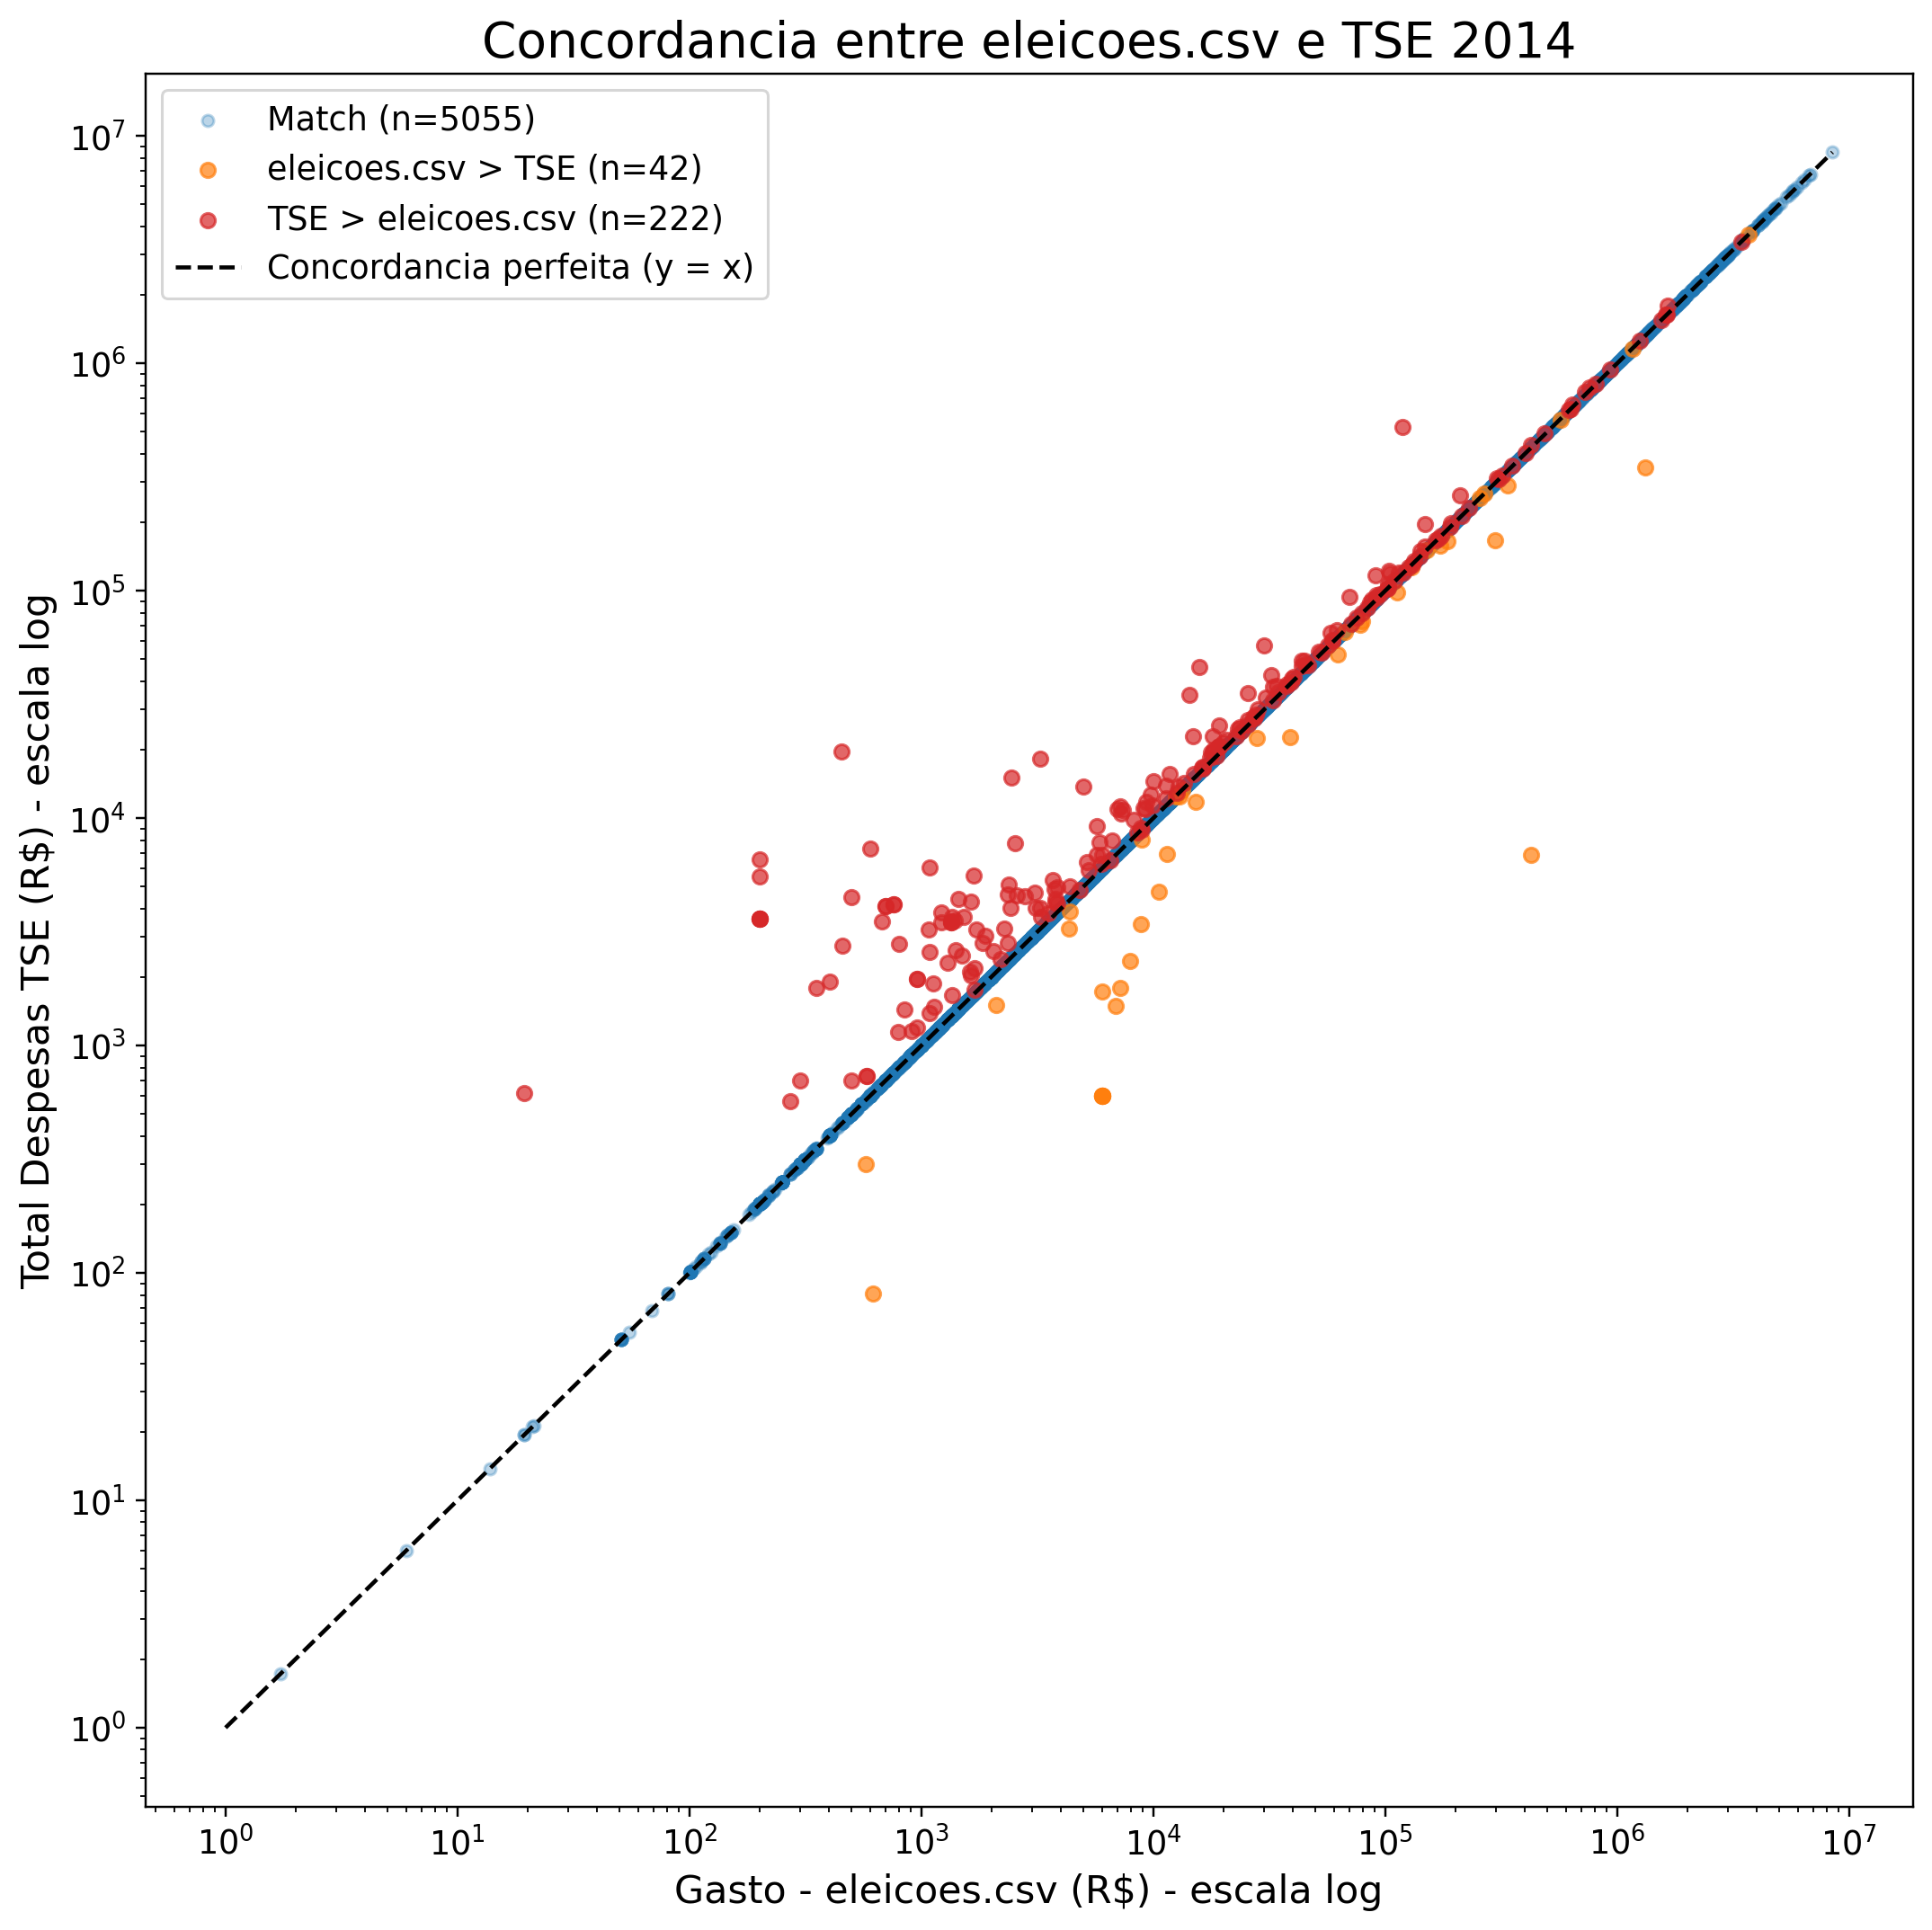
\includegraphics[width=0.98\columnwidth]{validacao_gasto_tse.png}
  \caption{Comparação entre o gasto do dataset original e o total apurado no TSE.}
  \label{fig:validacao}
\end{figure}

\subsection{Caracterização Inicial do Dataset Enriquecido}

O processo de preparação resultou em um dataset analítico com 6.353
candidaturas distribuídas em 26 UFs presentes no arquivo original e 32
partidos distintos. As variáveis de gênero, raça e situação eleitoral foram
recuperadas para 6.349 registros, o que garante cobertura quase completa para
as análises complementares de representatividade. Além disso, a base auxiliar
de fornecedores reuniu 366.289 registros de despesas, permitindo observar não
apenas quanto cada candidato gastou, mas também para onde os recursos foram
transferidos.

Essa ampliação é importante porque transforma o problema original, centrado
apenas em votos e dinheiro, em uma base mais rica para examinar desigualdade,
intermediação partidária e estrutura econômica das campanhas. Assim, o artigo
mantém o núcleo exigido pelo briefing, mas passa a interpretar o fenômeno
com maior profundidade substantiva. A Figura~\ref{fig:validacao} mostra que
a maior parte dos pontos permanece muito próxima da diagonal, o que indica
boa concordância entre o gasto agregado no arquivo original e o total
recuperado nas bases do TSE. O gráfico auxiliar de divergências por UF,
gerado no notebook, reforça que as discrepâncias relevantes se concentram em
poucos estados e não alteram o padrão descritivo central utilizado no artigo.

\subsection{Panorama Nacional do Dataset}

Após a filtragem por gasto positivo, restaram 5.323 candidaturas para análise
de financiamento. A média nacional de gasto foi de R\$ 220.397, enquanto a
mediana foi de apenas R\$ 9.916, diferença que evidencia forte assimetria à
direita. O gasto máximo observado ultrapassou R\$ 8,4 milhões. Em votos, a
mediana nacional entre candidatos com gasto e votos positivos foi de 1.772,
frente a média de 18.045.

\begin{figure}[H]
  \centering
  \tablePlaceholder{Inserir screenshot da Tabela 3.1 do notebook.}
  \caption{Estatísticas descritivas do dataset nacional de eleições 2014.}
  \label{tab:descritivas_brasil}
\end{figure}

\begin{figure}[H]
  \centering
  
\includegraphics[width=0.98\columnwidth]{distribuicao_gasto.png}
  \caption{Distribuição nacional do gasto de campanha.}
  \label{fig:distribuicao_gasto_brasil}
\end{figure}

A Figura~\ref{fig:distribuicao_gasto_brasil} mostra uma distribuição
fortemente assimétrica à direita: a maioria das candidaturas se concentra em
baixos níveis de gasto, enquanto uma minoria ocupa a cauda longa de valores
muito elevados. Essa configuração explica o distanciamento entre média e
mediana e reforça a adequação da escala logarítmica para esse tipo de dado.

\begin{figure}[H]
  \centering
  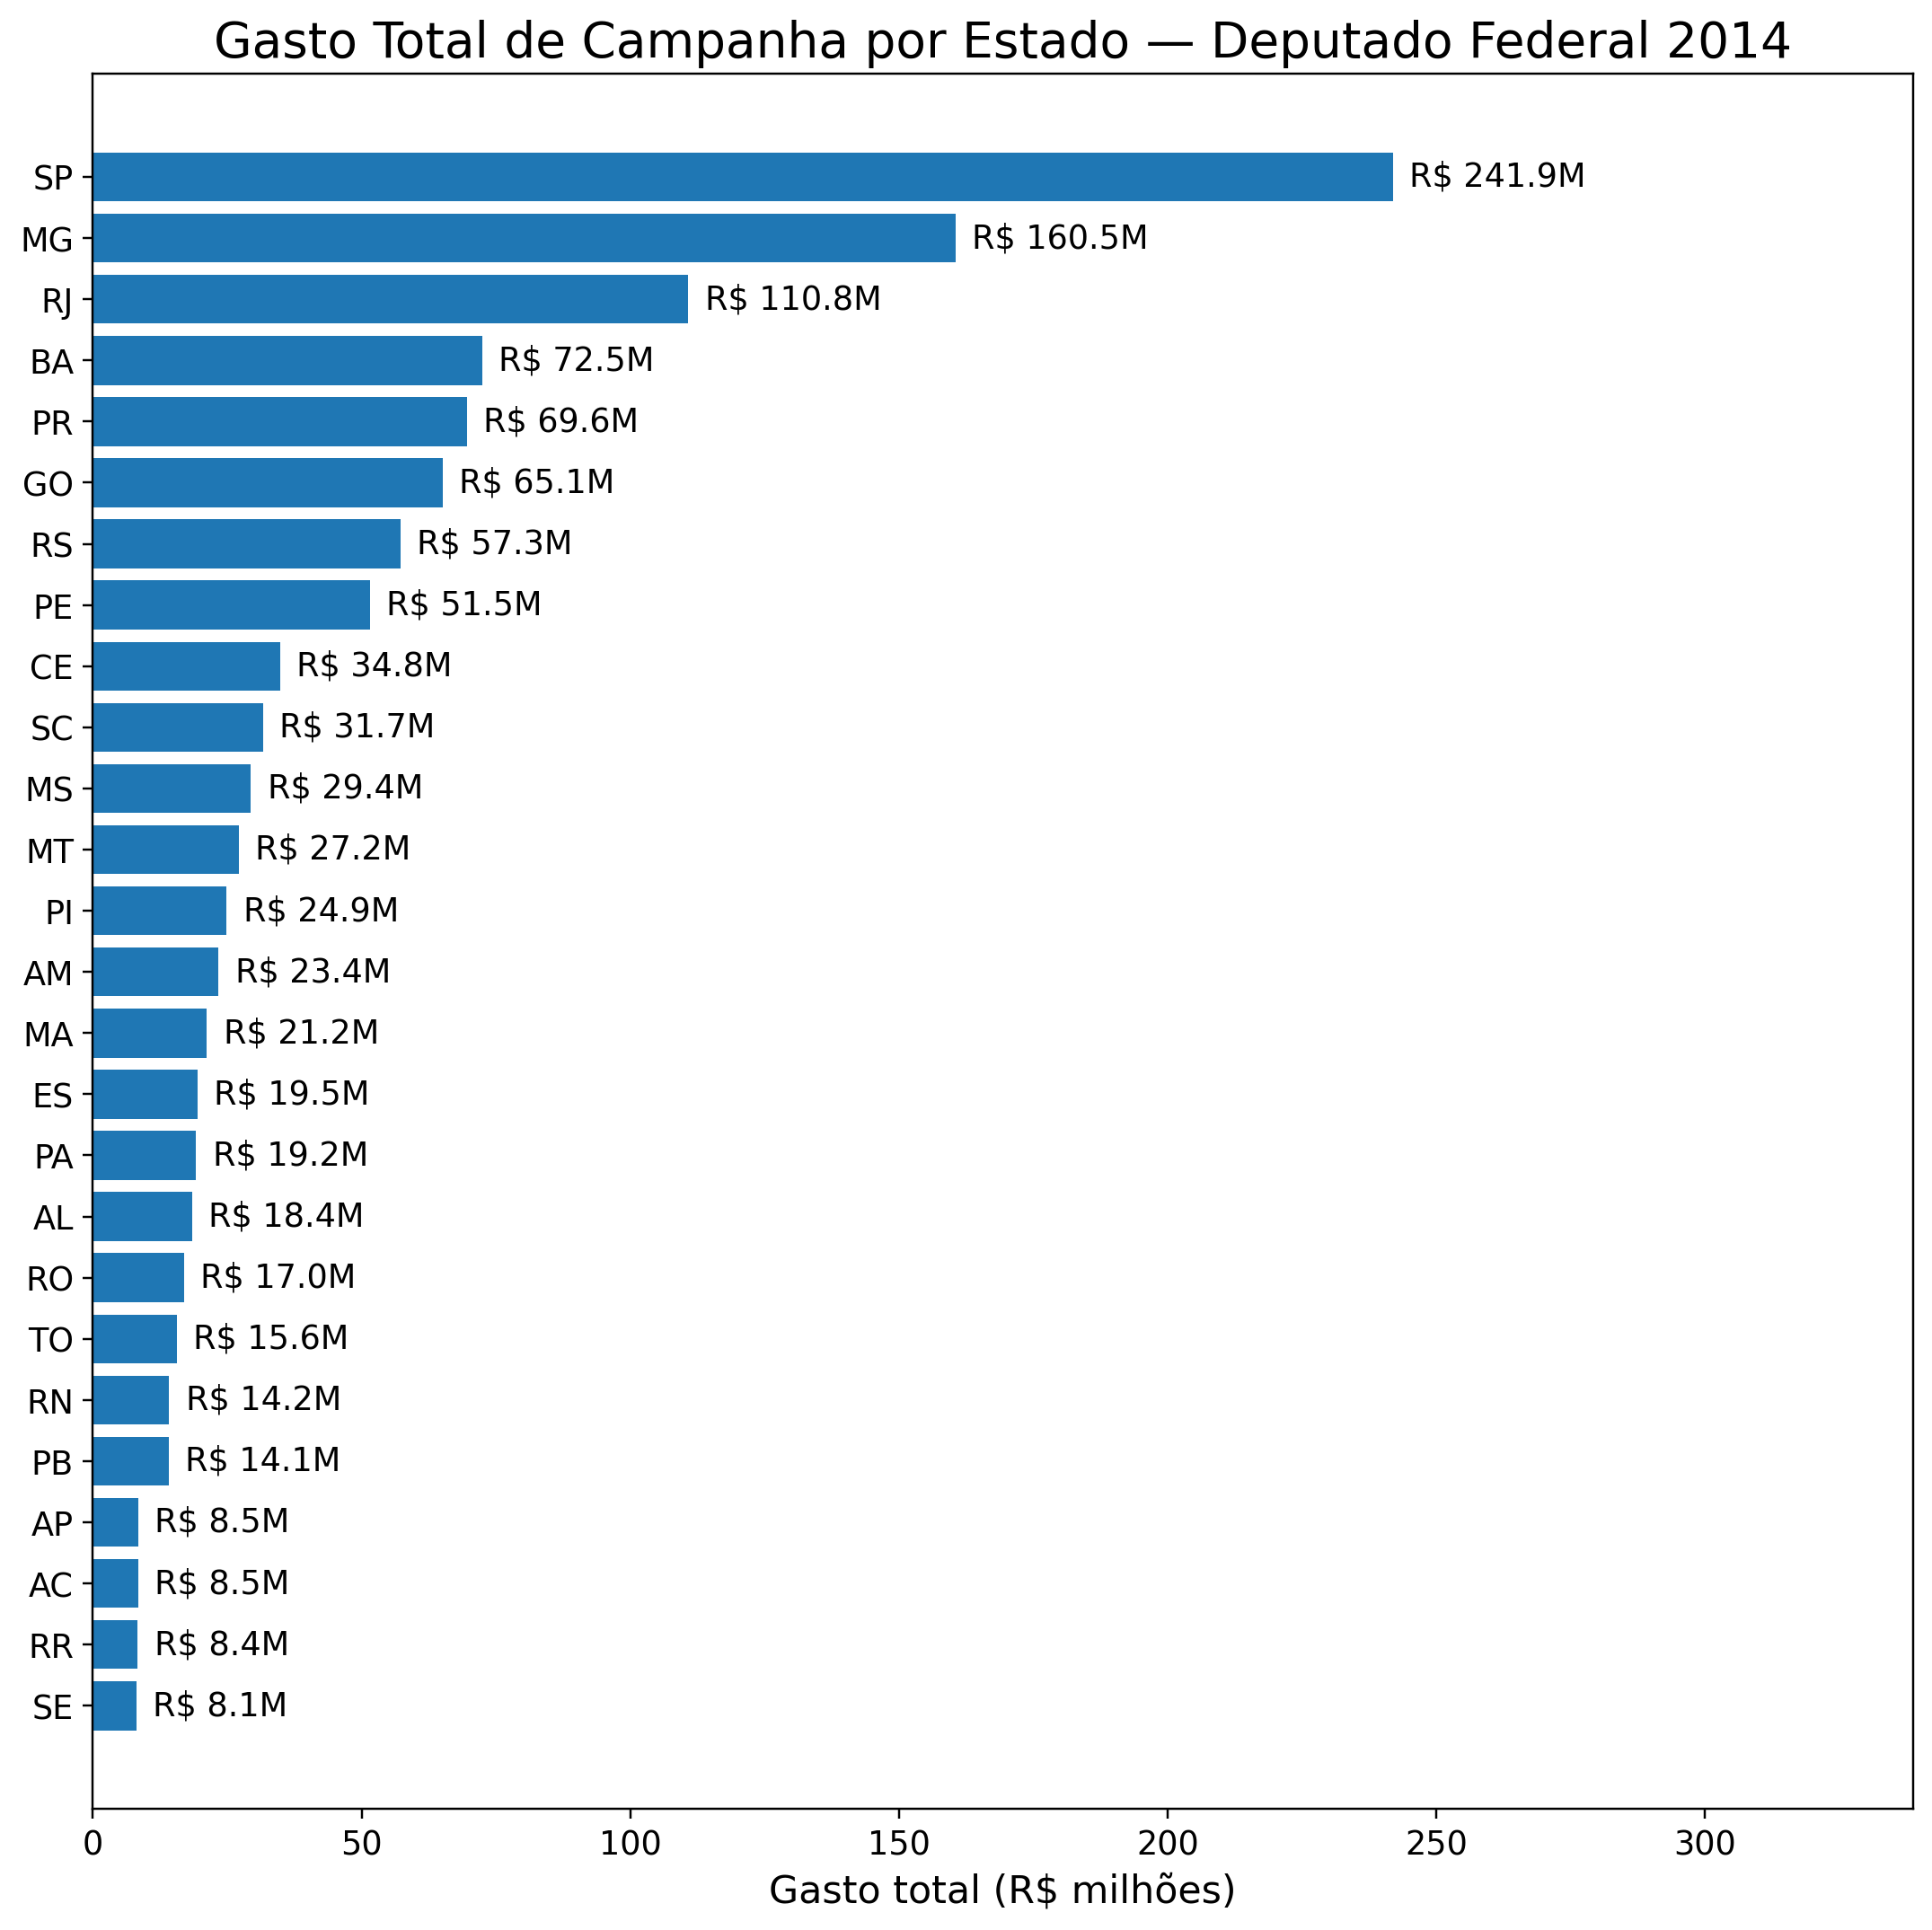
\includegraphics[width=0.98\columnwidth]{gasto_total_estado.png}
  \caption{Top estados por gasto total de campanha.}
  \label{fig:gasto_total_estado}
\end{figure}

No agregado nacional, SP, MG e RJ concentram os maiores volumes absolutos de
gasto, o que reflete o peso eleitoral e demográfico dessas UFs. Em termos
substantivos, esse ranking capta o tamanho do mercado político em cada estado,
e não necessariamente o padrão do candidato típico.

\begin{figure}[H]
  \centering
  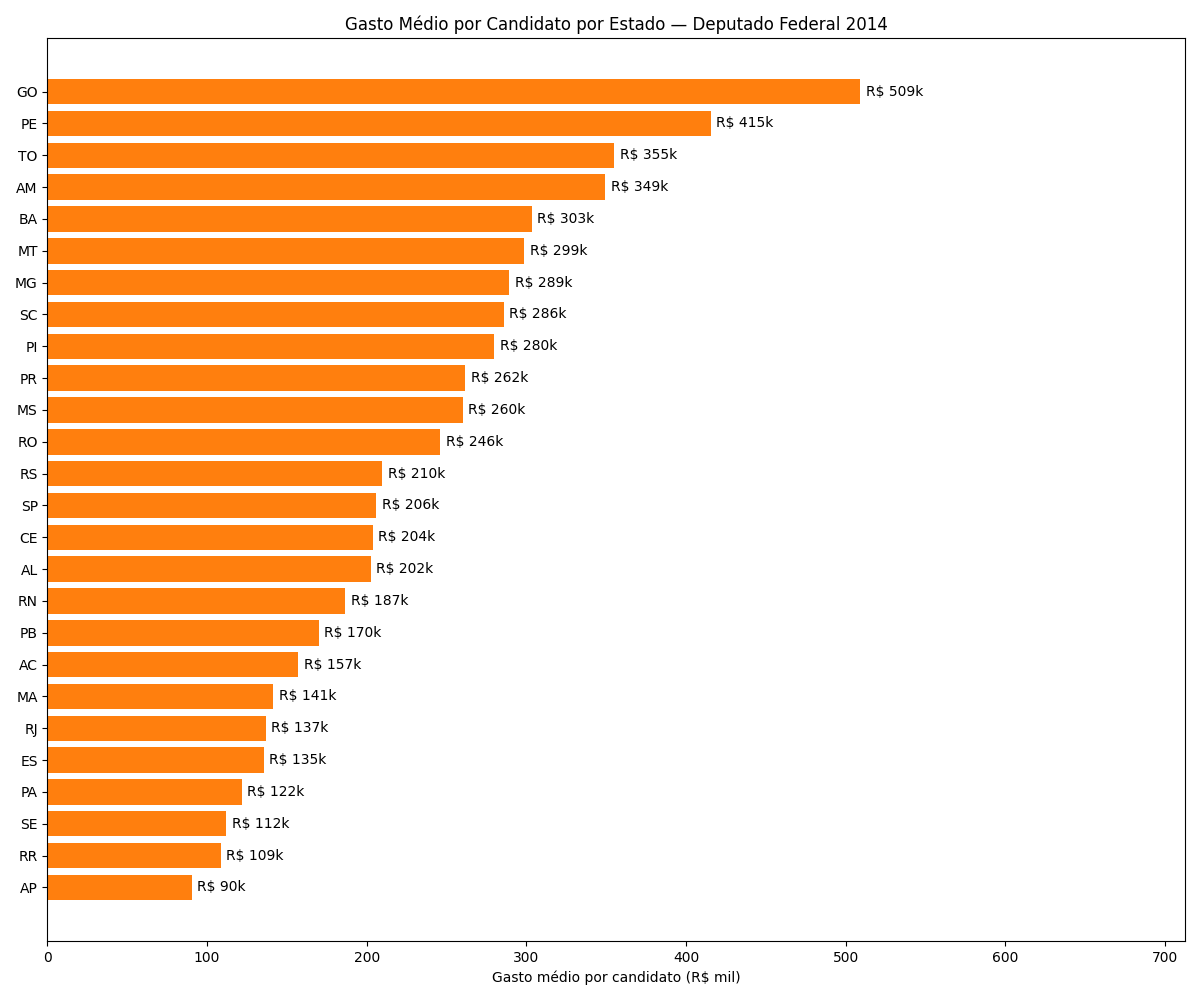
\includegraphics[width=0.98\columnwidth]{gasto_medio_estado.png}
  \caption{Top estados por gasto médio por candidatura.}
  \label{fig:gasto_medio_estado}
\end{figure}

Quando se observa gasto médio por candidatura, o ordenamento muda: estados
menores passam a ocupar posições superiores, indicando campanhas mais
concentradas em poucos nomes ou menor dispersão de recursos entre candidaturas.
Esse contraste entre total e média mostra que as duas métricas capturam
fenômenos distintos: escala agregada do financiamento e intensidade média de
investimento por candidato.

\subsection{Estrutura Partidária do Financiamento}

A distribuição dos recursos entre partidos ajuda a entender como o gasto de
campanha se organiza politicamente no plano nacional. Quando se observa o
valor total investido, partidos grandes e competitivos concentram mais
recursos absolutos.

\begin{figure}[H]
  \centering
  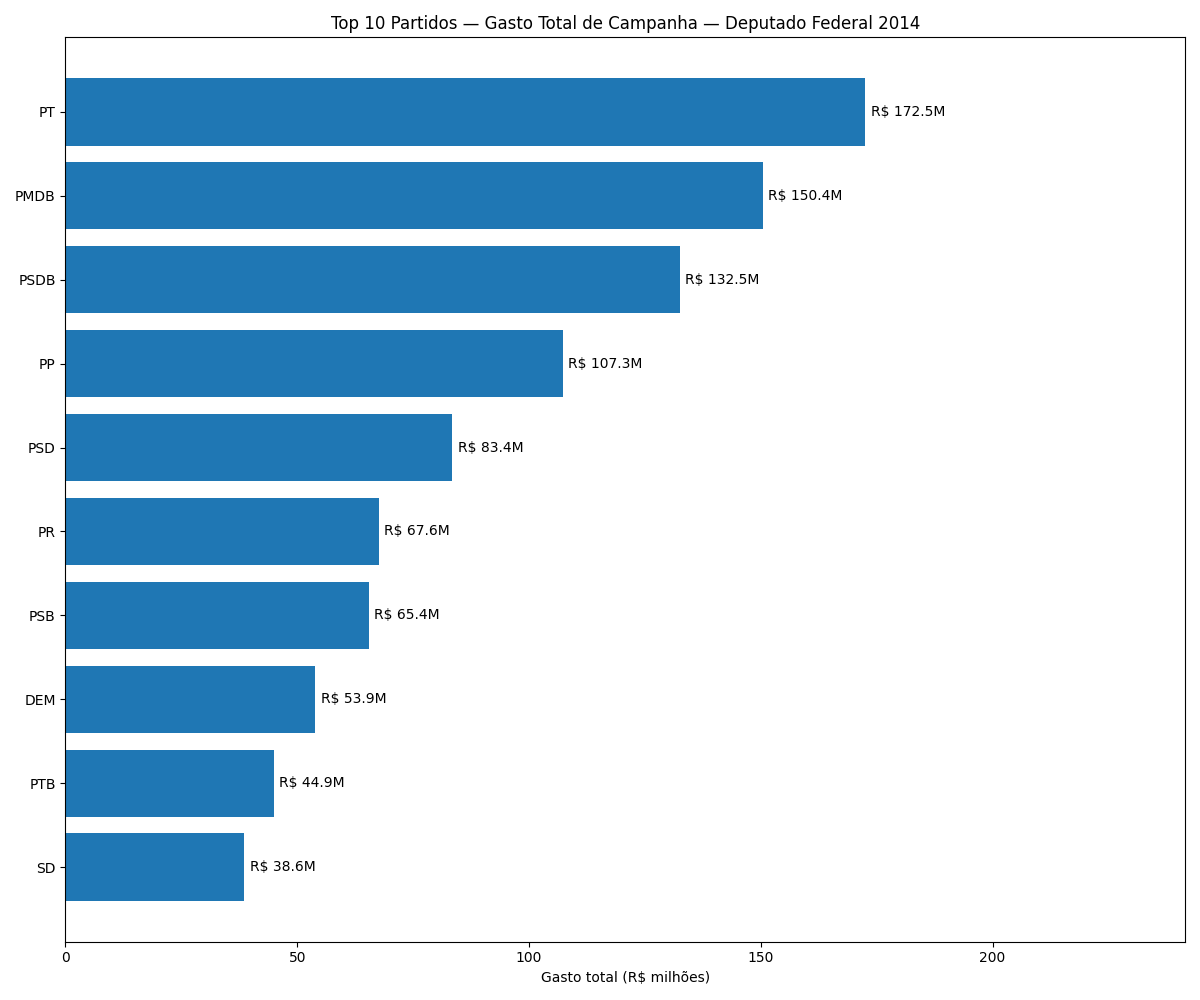
\includegraphics[width=0.98\columnwidth]{gasto_total_partido.png}
  \caption{Top partidos por gasto total de campanha.}
  \label{fig:partidos_total}
\end{figure}

No ranking de gasto total, PT, PMDB, PSDB e PP aparecem entre os principais
partidos de 2014, refletindo capilaridade nacional, presença em múltiplas UFs
e maior capacidade de financiamento. Esse gráfico resume melhor a dimensão
agregada do sistema partidário do que uma simples contagem de candidaturas,
pois mostra quais siglas efetivamente concentraram mais recursos no ciclo.

Quando a análise passa do total para a média por candidatura, a leitura muda:
aí aparecem com mais força estratégias de concentração, nas quais poucos nomes
recebem valores muito superiores à média nacional.

\begin{figure}[H]
  \centering
  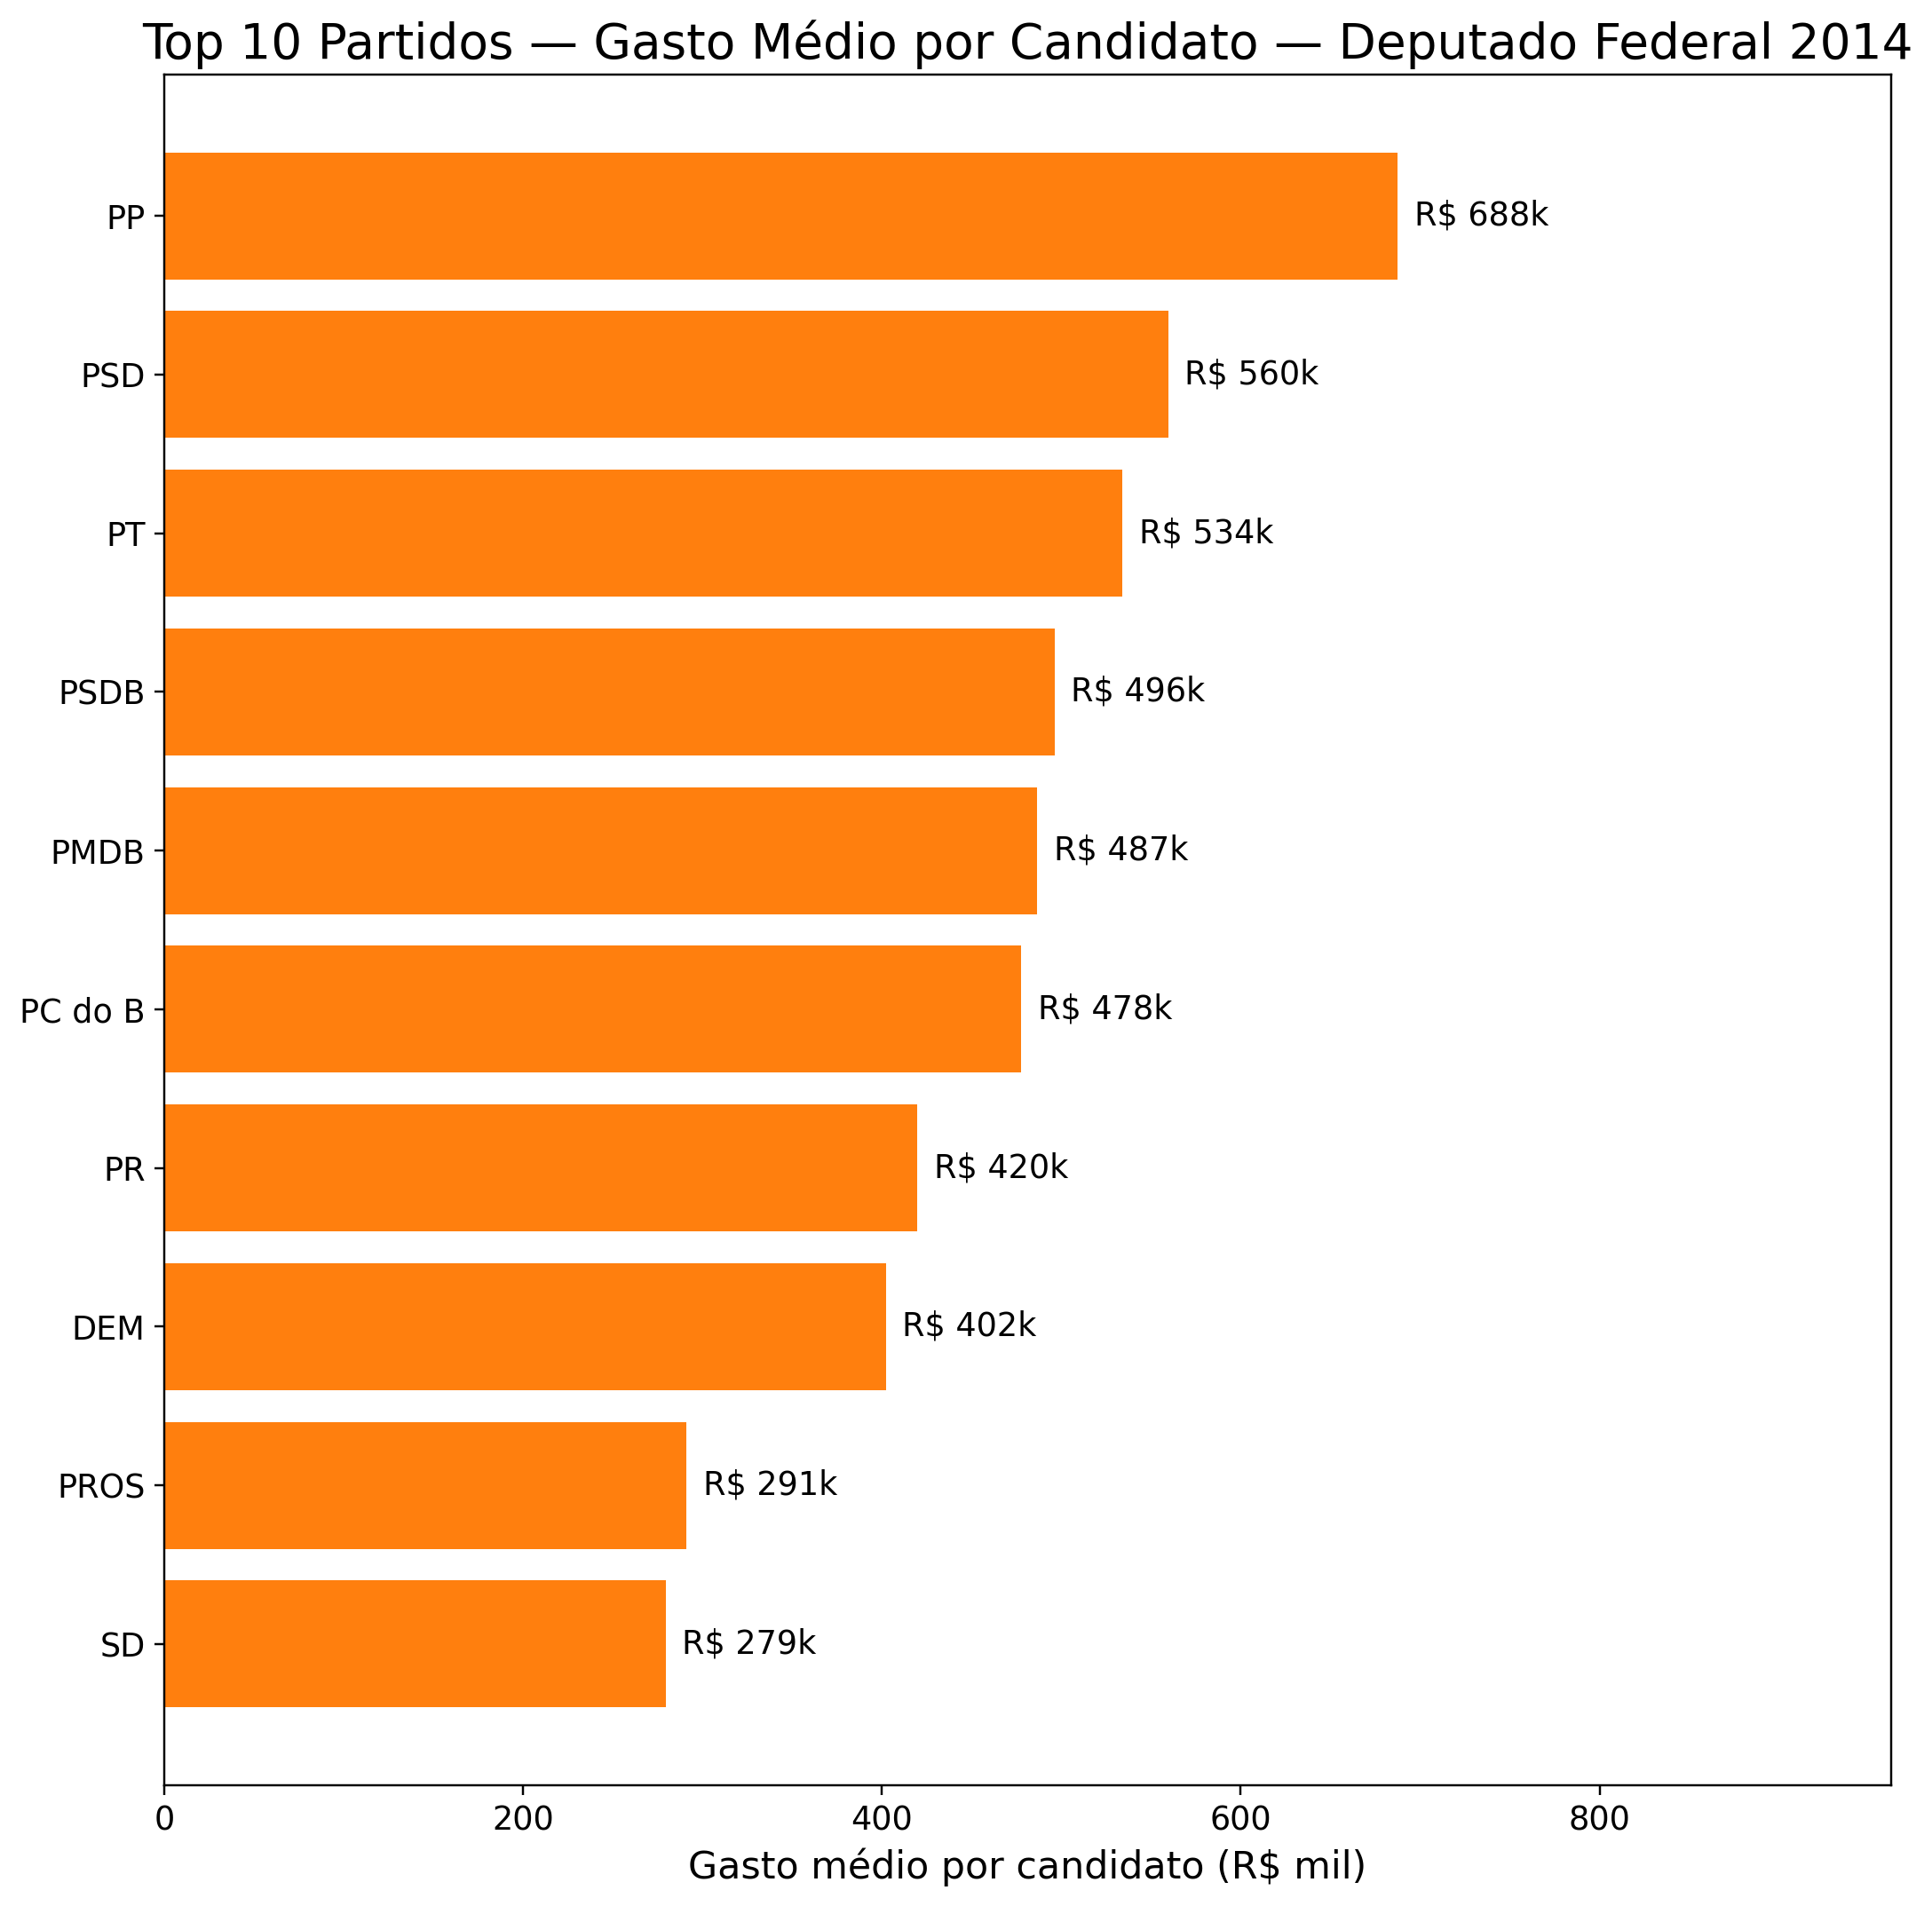
\includegraphics[width=0.98\columnwidth]{gasto_medio_partido.png}
  \caption{Top partidos por gasto médio por candidatura.}
  \label{fig:partidos_medio}
\end{figure}

A Figura~\ref{fig:partidos_medio} revela outra lógica de organização do
financiamento. Partidos com menos candidaturas podem subir no ranking ao
concentrarem recursos em poucos nomes competitivos. Em conjunto, os dois
indicadores mostram que volume agregado e intensidade média de investimento
são dimensões complementares, mas não equivalentes, da estrutura partidária.

\subsection{Gasto versus Votos no Brasil}

O gráfico de dispersão nacional mostra que candidatos eleitos se concentram,
em geral, no quadrante superior direito, combinando mais gasto e mais votos.
Também se observa uma faixa de gasto abaixo da qual a eleição se torna rara,
o que sugere a existência de um patamar mínimo de visibilidade eleitoral.

\begin{figure}[H]
  \centering
  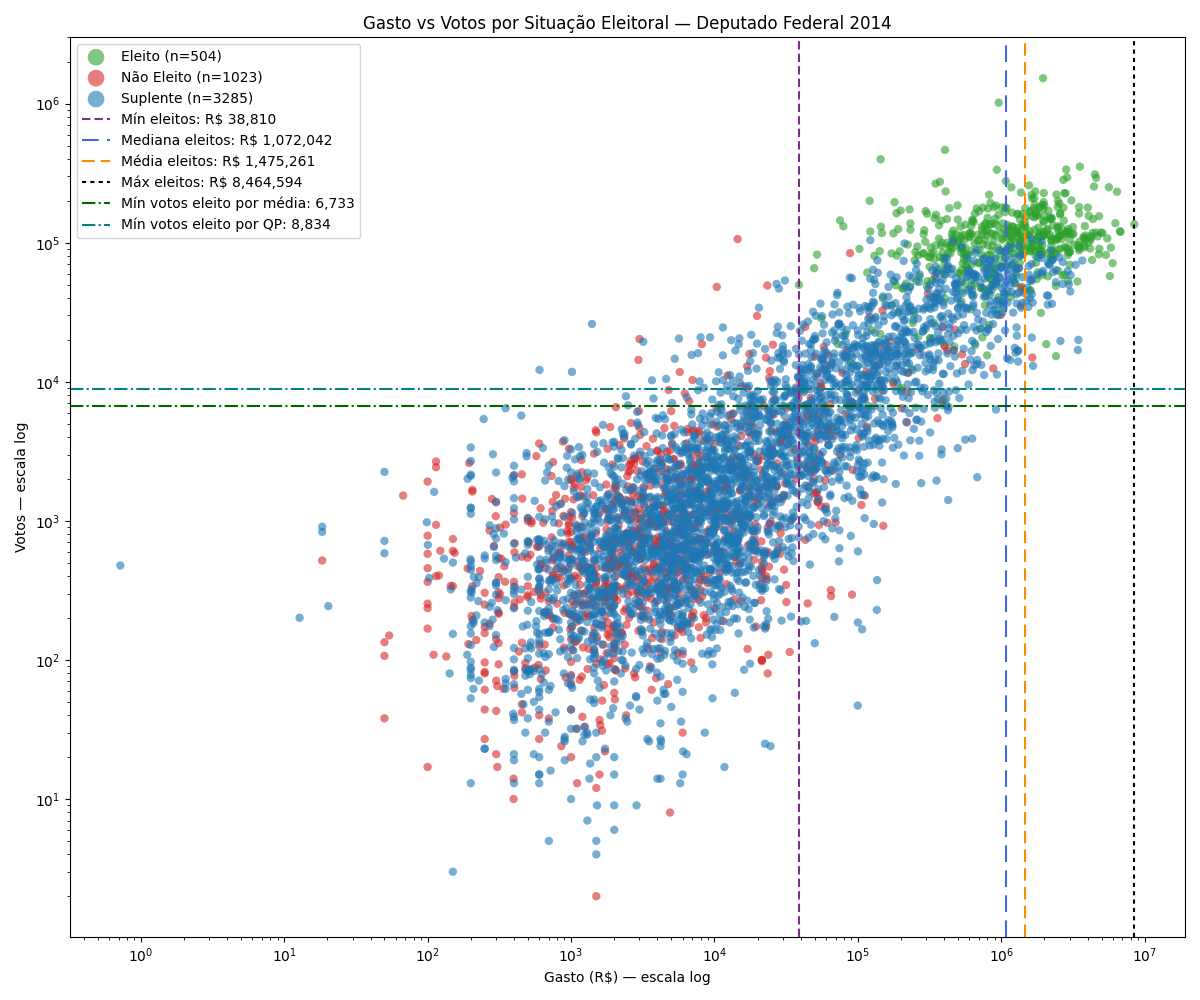
\includegraphics[width=0.98\columnwidth]{gasto_vs_votos.png}
  \caption{Dispersão nacional entre gasto de campanha e votos.}
  \label{fig:brasil_disp}
\end{figure}

O coeficiente de Pearson nacional foi $r = 0{,}593$, caracterizando
correlação moderada positiva. Em termos substantivos, isso significa que mais
dinheiro tende a estar associado a mais votos, mas o gasto, isoladamente, não
explica todo o desempenho eleitoral. A matriz de correlação gerada no notebook
foi omitida do artigo por ser redundante em relação ao coeficiente já
reportado no texto e à própria estrutura visual do gráfico de dispersão.

\subsection{Requisitos Obrigatórios do Briefing: Três Estados}

As subseções seguintes cobrem integralmente o item obrigatório do professor
para três UFs escolhidas: histogramas de gasto e votos, além do gráfico de
dispersão com correlação de Pearson.

\subsubsection{Rio de Janeiro (RJ)}

No RJ, 810 candidaturas registraram gasto positivo. A distribuição de gasto é
fortemente assimétrica à direita, com mediana de R\$ 6.024 frente a média de
R\$ 136.771.

\begin{figure}[H]
  \centering
  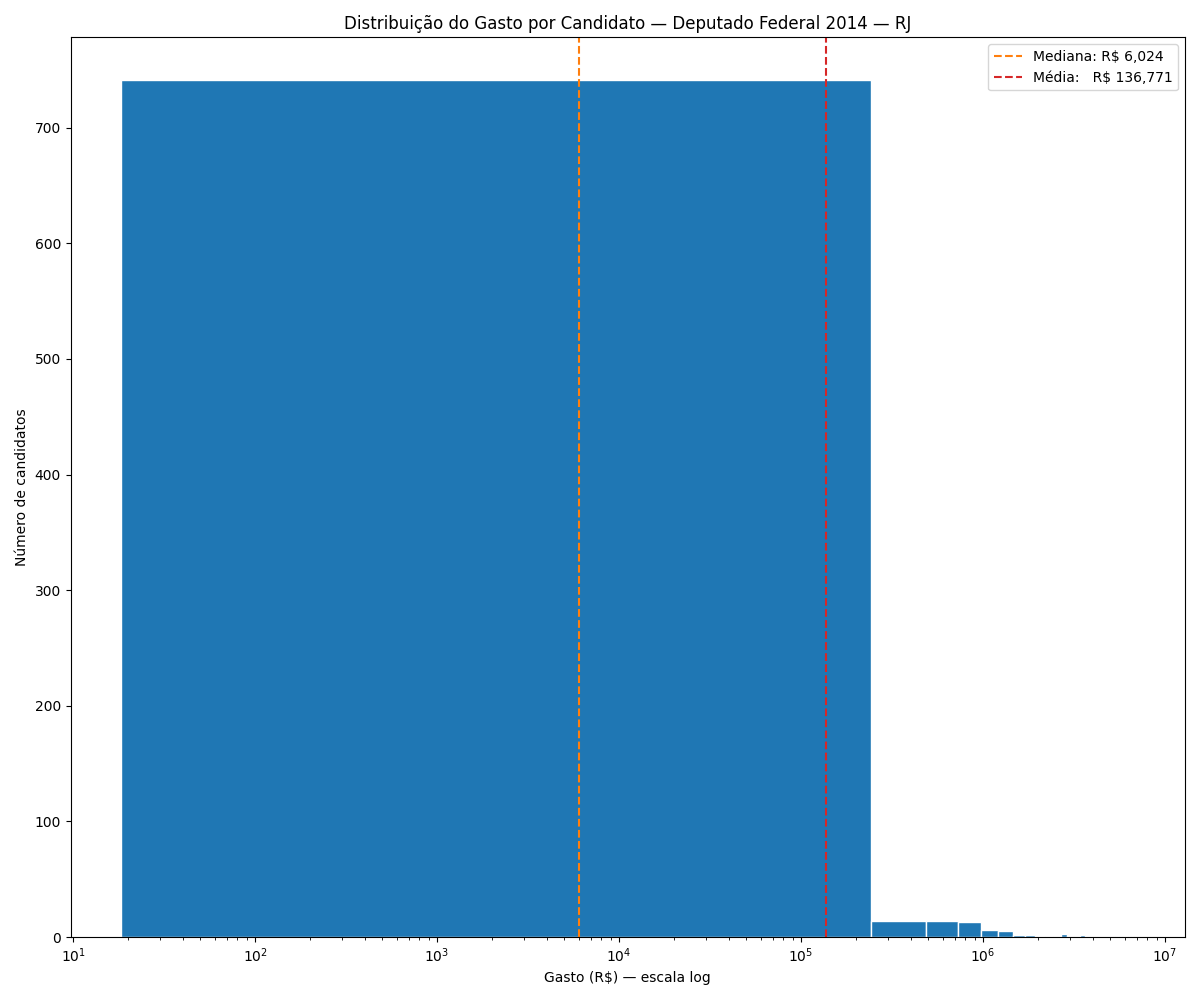
\includegraphics[width=0.98\columnwidth]{rj_distribuicao_gasto.png}
  \caption{Histograma do gasto de campanha no Rio de Janeiro.}
  \label{fig:rj_gasto}
\end{figure}

A Figura~\ref{fig:rj_gasto} mostra que a maior parte dos candidatos se
concentra em níveis baixos de gasto, enquanto poucos nomes ocupam a cauda de
valores muito elevados. A diferença entre mediana e média confirma que o
comportamento típico da candidatura fluminense está muito abaixo do nível de
investimento dos casos extremos.

A distribuição de votos no estado também apresenta cauda longa, com muitos
casos em baixas contagens e poucos candidatos concentrando centenas de milhares
de votos.

\begin{figure}[H]
  \centering
  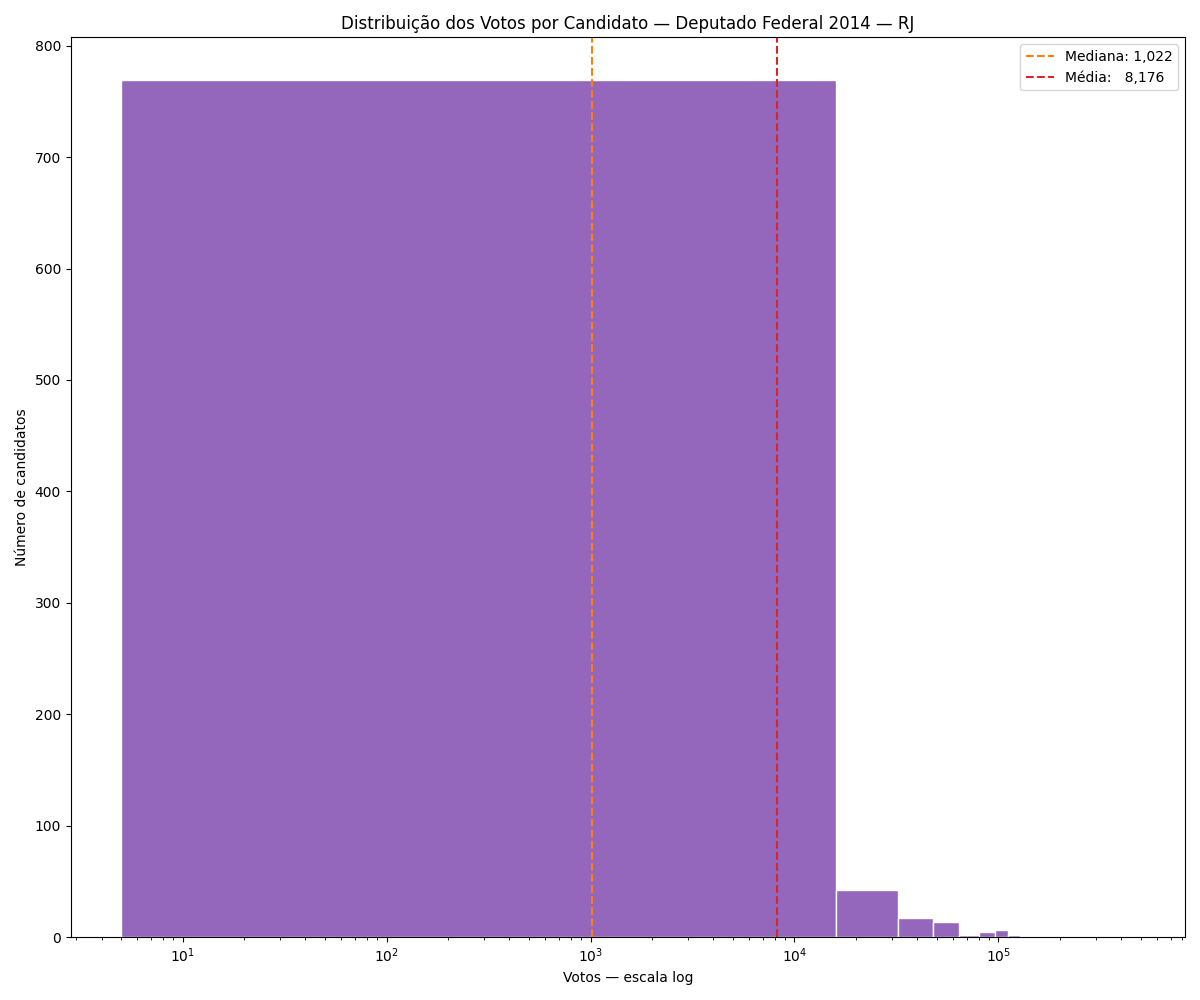
\includegraphics[width=0.98\columnwidth]{rj_distribuicao_votos.png}
  \caption{Histograma dos votos no Rio de Janeiro.}
  \label{fig:rj_votos}
\end{figure}

A Figura~\ref{fig:rj_votos} reforça a natureza altamente concentrada da disputa:
a maioria das candidaturas recebe poucos votos, enquanto um grupo reduzido se
descola fortemente da massa principal. Em termos descritivos, a assimetria dos
votos acompanha a assimetria do financiamento.

\begin{figure}[H]
  \centering
  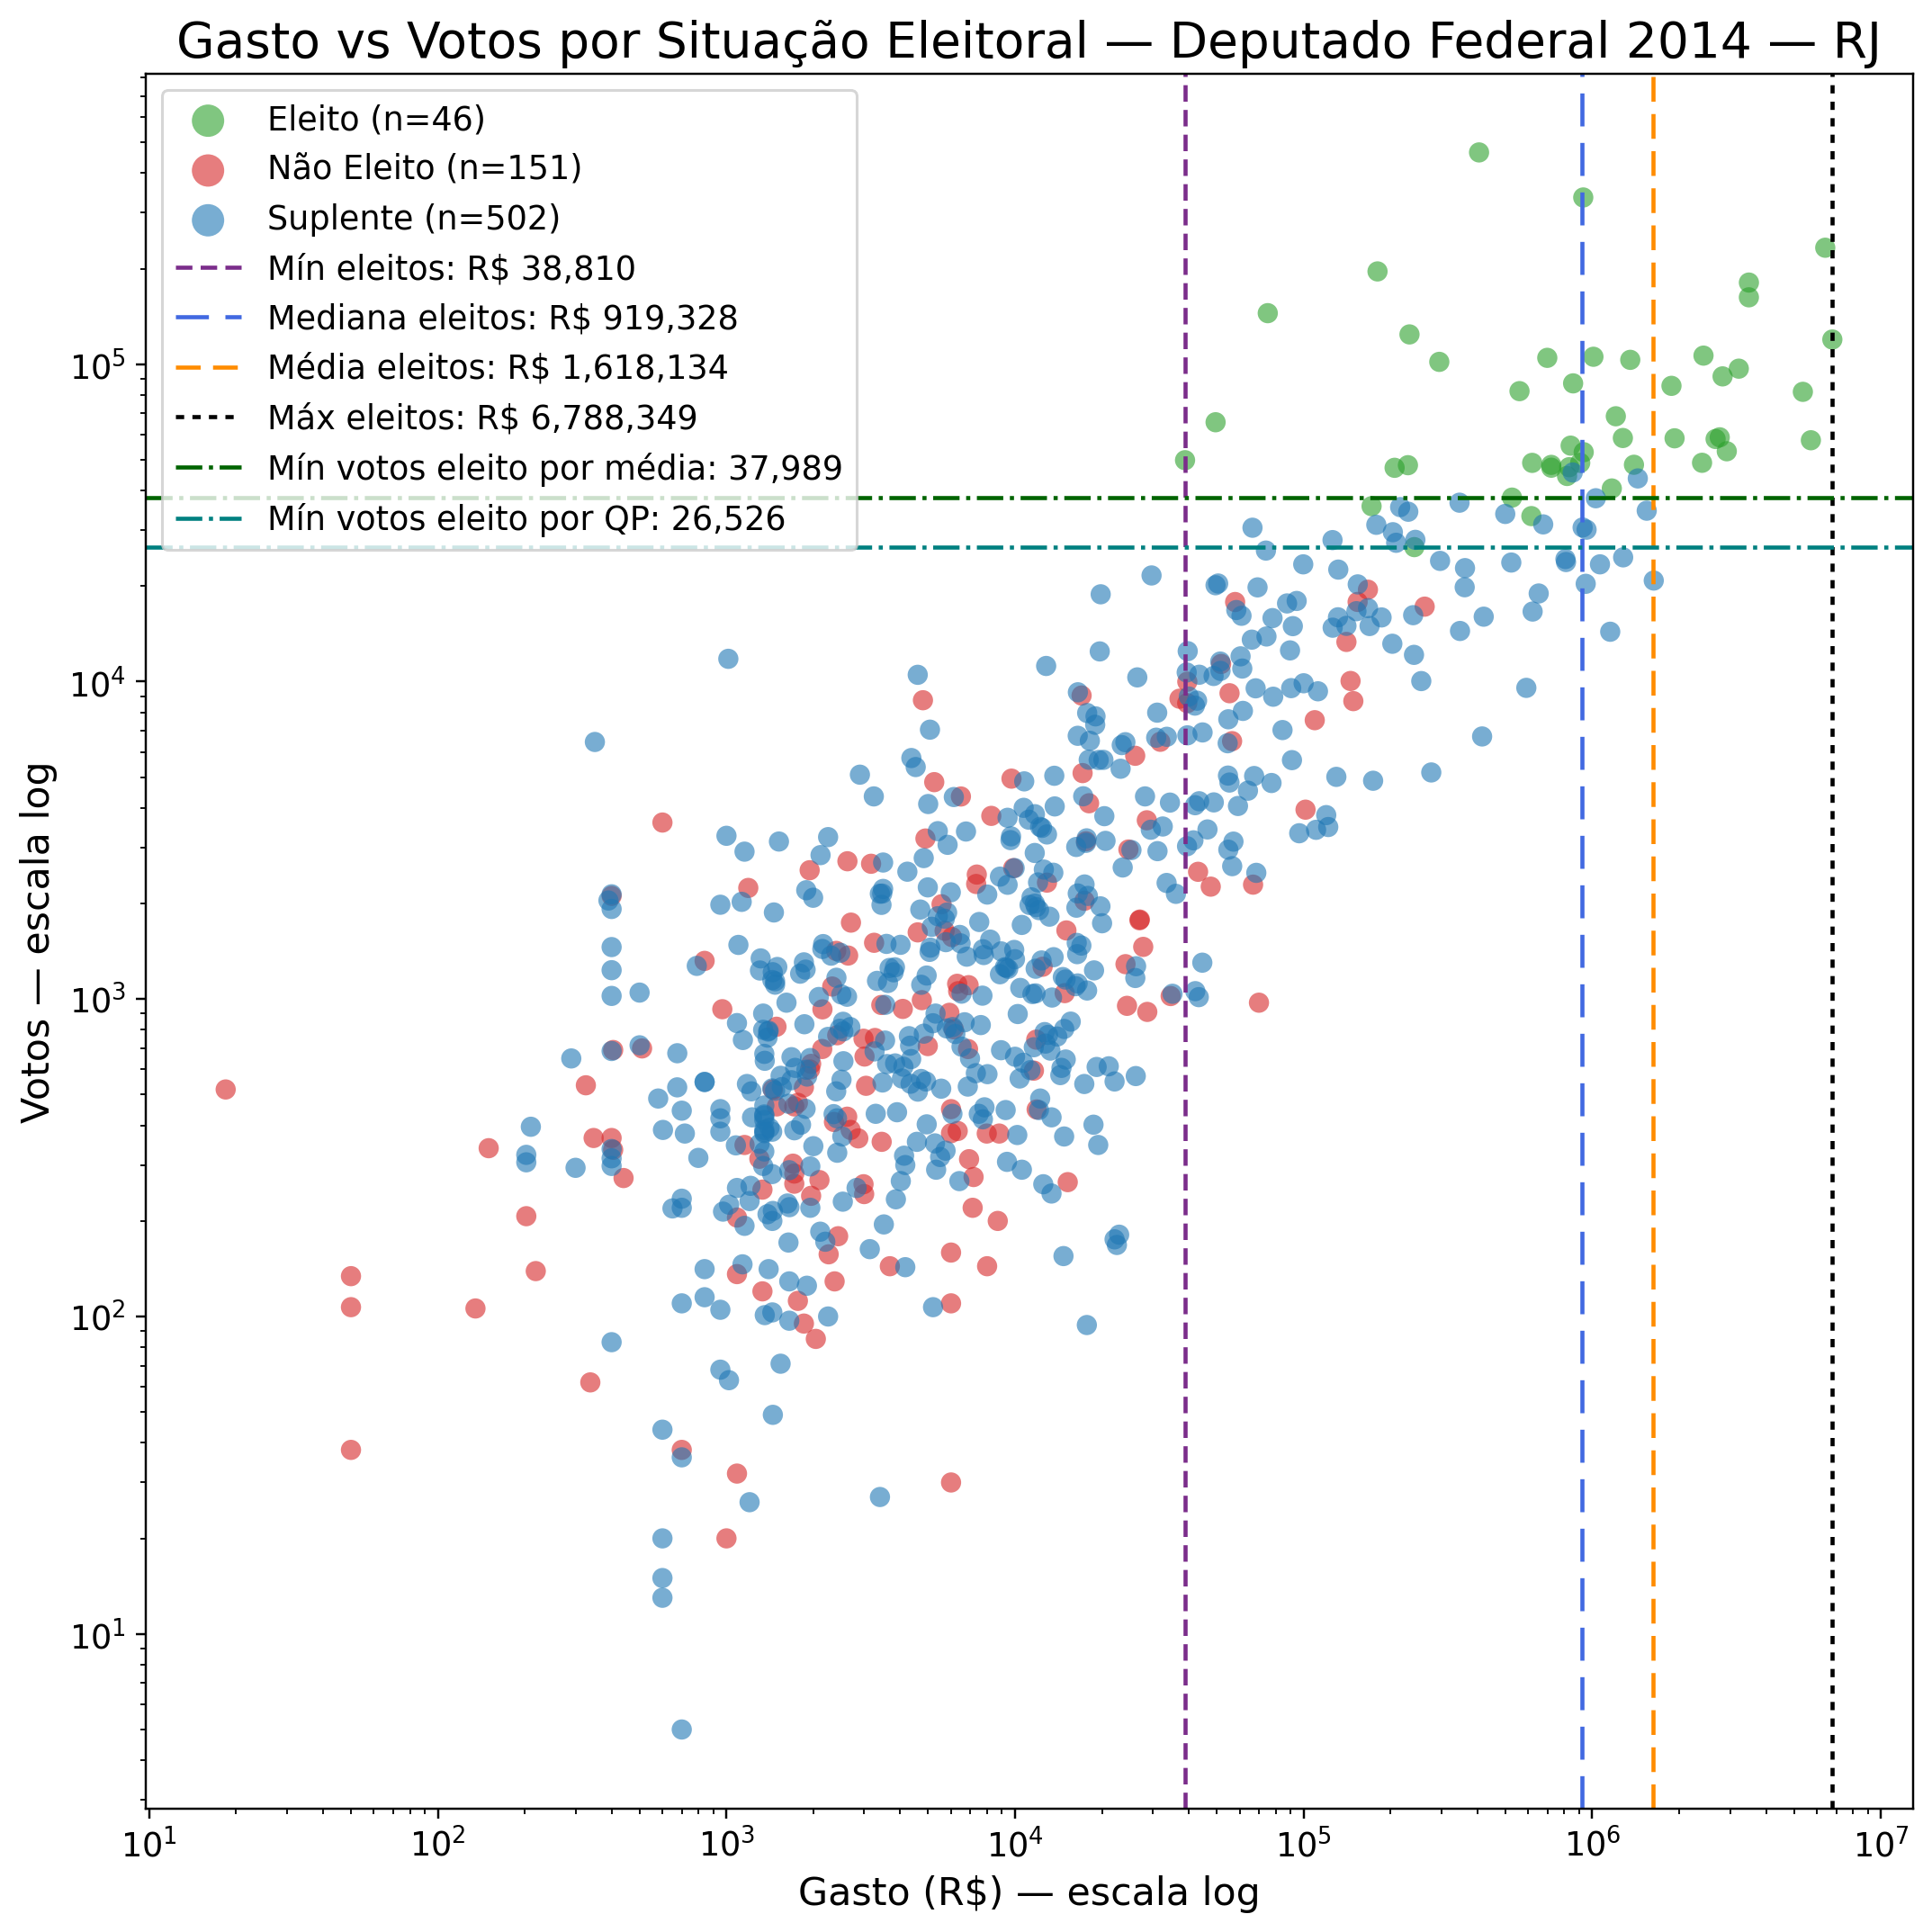
\includegraphics[width=0.98\columnwidth]{gasto_vs_votos_RJ.png}
  \caption{Dispersão entre gasto e votos no Rio de Janeiro.}
  \label{fig:rj_disp}
\end{figure}

O coeficiente de Pearson no RJ foi $r = 0{,}556$, indicando correlação
moderada positiva. Na Figura~\ref{fig:rj_disp}, a nuvem de pontos confirma a
tendência geral de aumento dos votos com o gasto, mas com dispersão
considerável e presença de candidatos que gastaram muito sem retorno
proporcional nas urnas. Ainda assim, observa-se separação razoável entre
candidatos eleitos e não eleitos.

\subsubsection{Goiás (GO)}

Em GO, 128 candidaturas tiveram gasto positivo. O estado apresenta um dos
quadros mais extremos de concentração: mediana de gasto de R\$ 4.048 e média
de R\$ 508.946.

\begin{figure}[H]
  \centering
  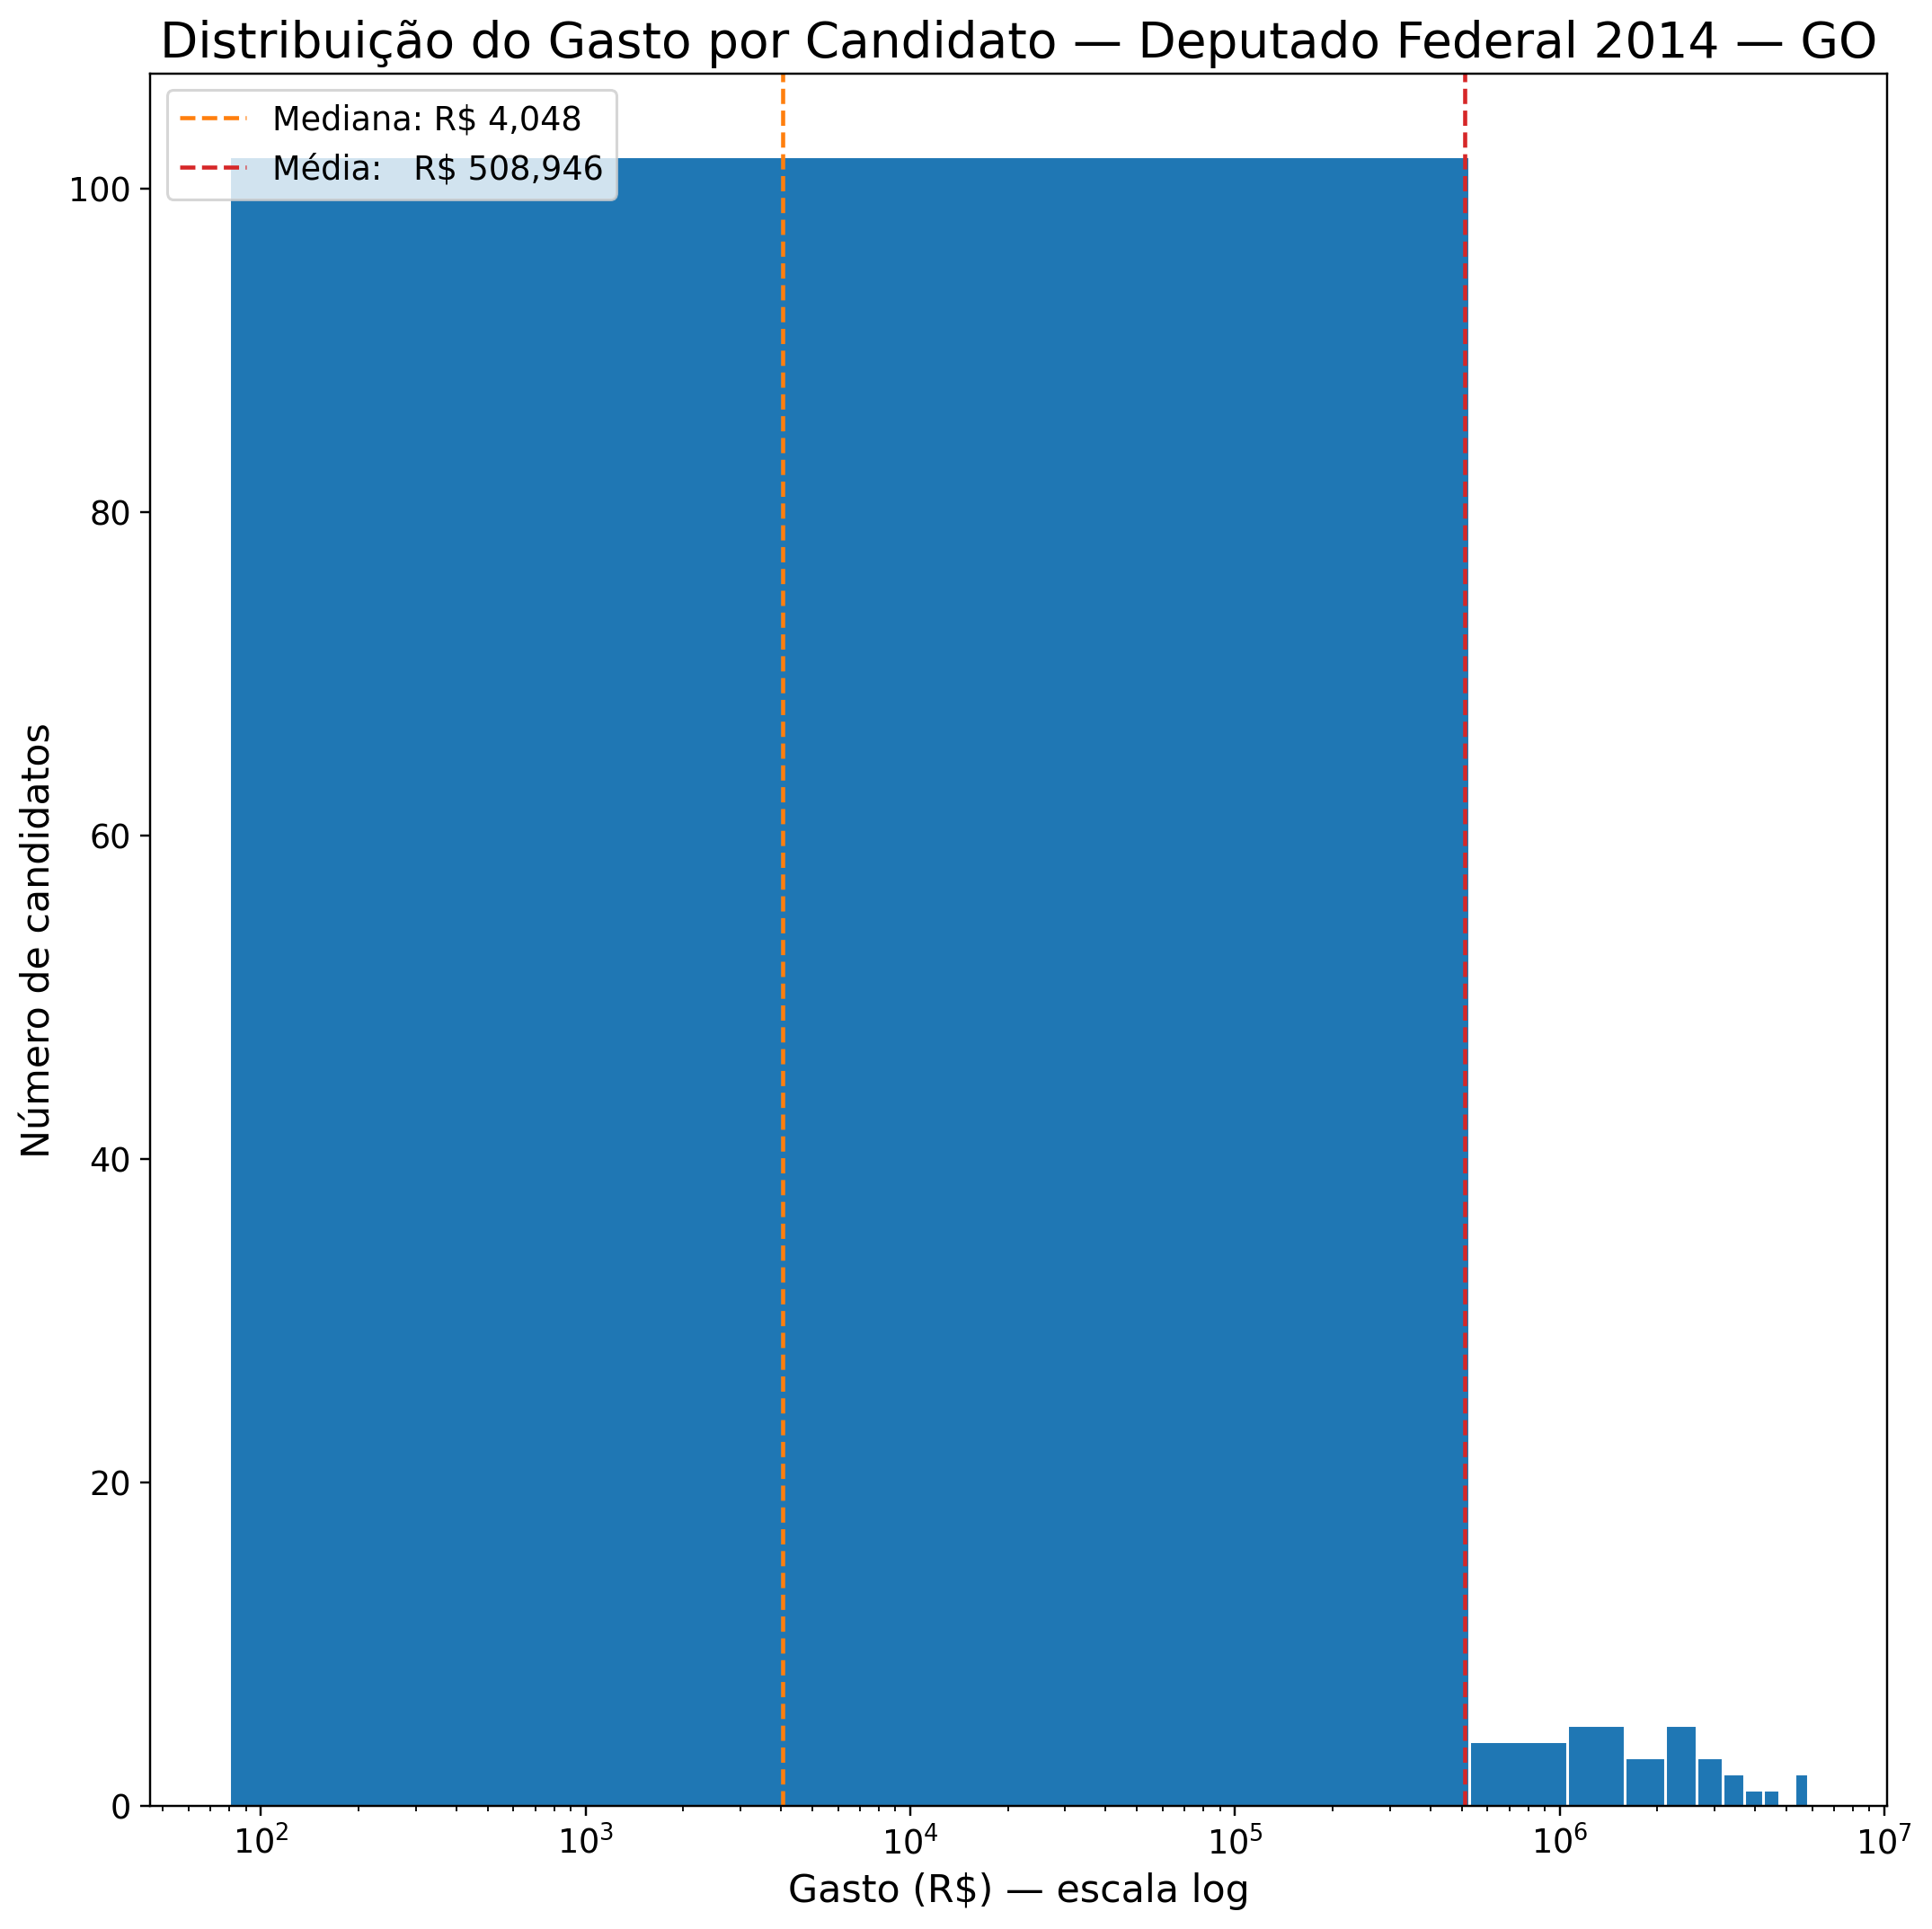
\includegraphics[width=0.98\columnwidth]{go_distribuicao_gasto.png}
  \caption{Histograma do gasto de campanha em Goiás.}
  \label{fig:go_gasto}
\end{figure}

A Figura~\ref{fig:go_gasto} mostra uma distribuição particularmente desigual,
na qual a massa das candidaturas permanece em níveis muito baixos de gasto,
enquanto poucos casos extremos deslocam fortemente a média. Esse padrão torna a
mediana uma descrição muito mais fiel do candidato típico no estado.

A distribuição de votos segue lógica semelhante, com concentração em baixos
valores e poucos candidatos muito acima do restante.

\begin{figure}[H]
  \centering
  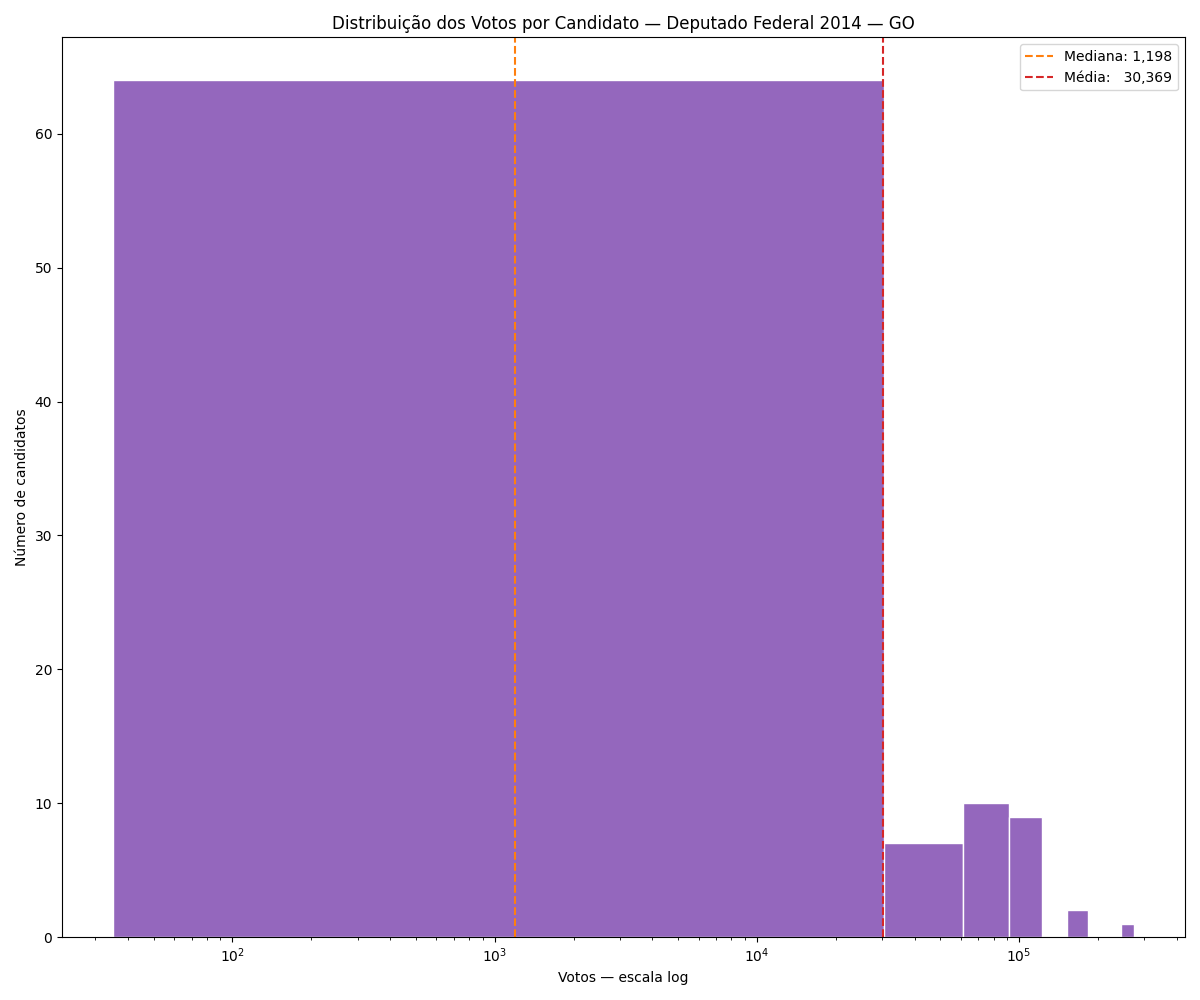
\includegraphics[width=0.98\columnwidth]{go_distribuicao_votos.png}
  \caption{Histograma dos votos em Goiás.}
  \label{fig:go_votos}
\end{figure}

Na Figura~\ref{fig:go_votos}, a cauda longa dos votos é ainda mais marcada do
que no RJ, refletindo o peso de um conjunto pequeno de candidatos altamente
competitivos em um estado com menos vagas e menos observações.

\begin{figure}[H]
  \centering
  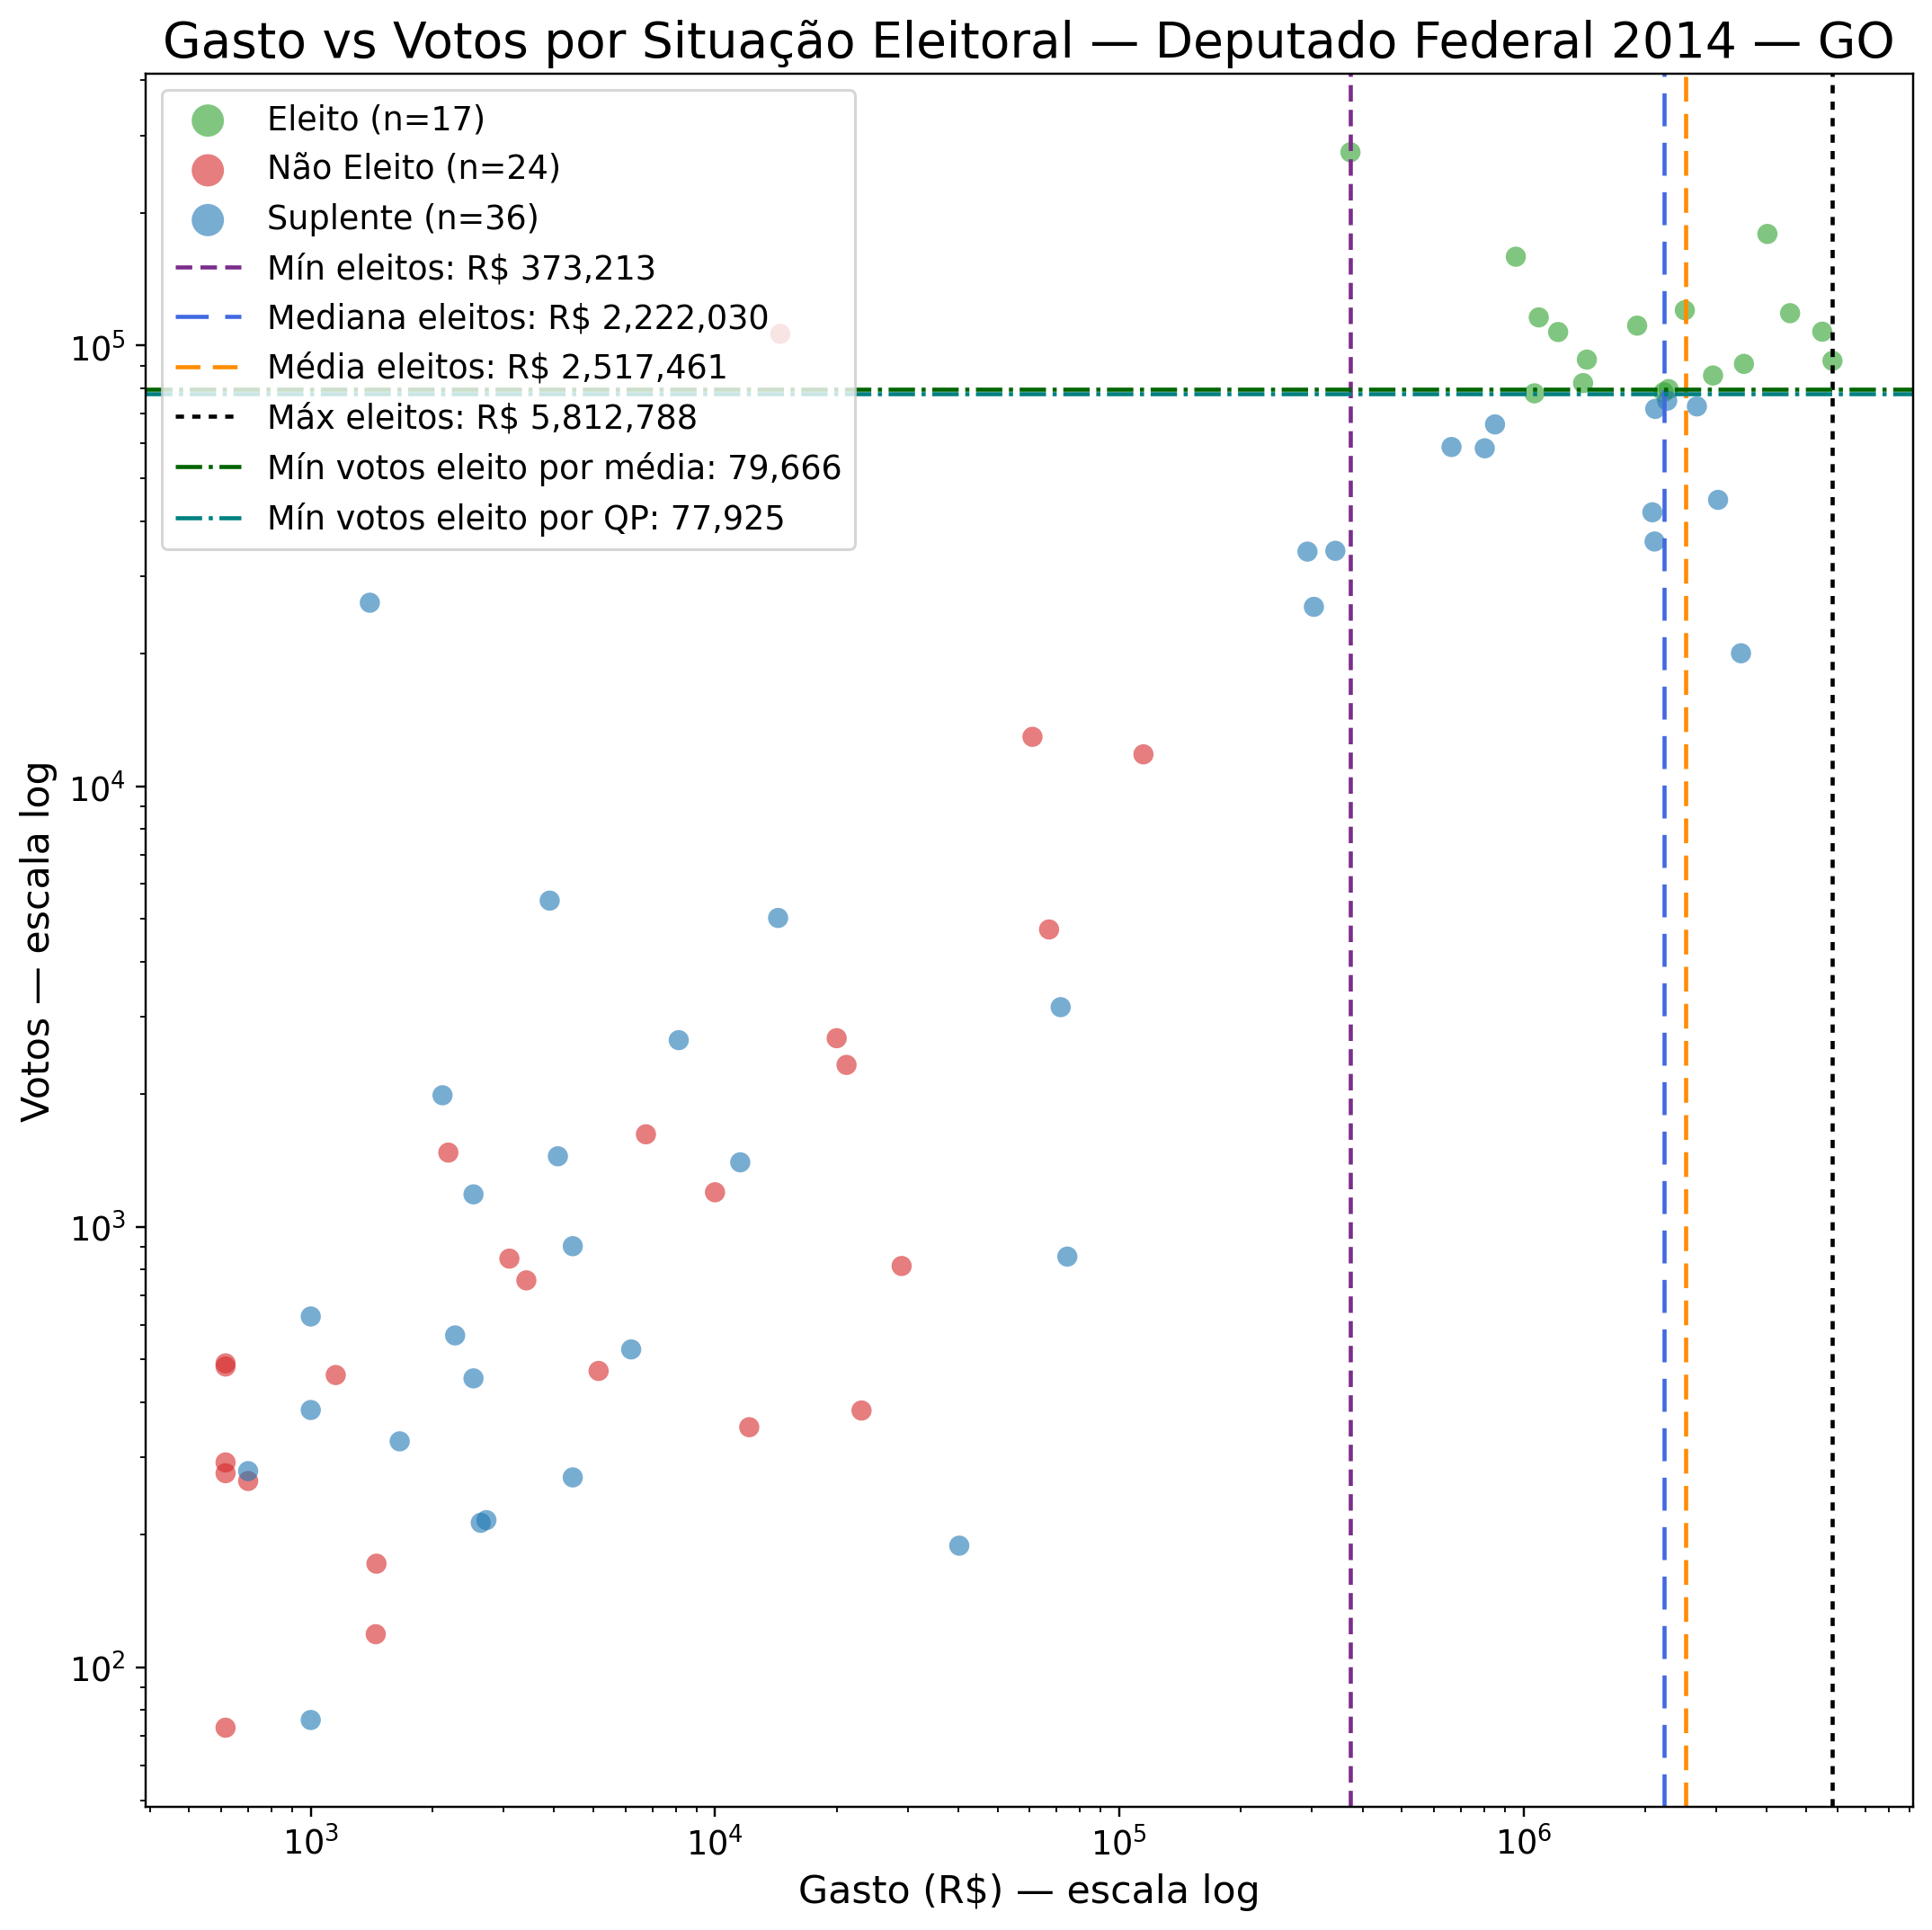
\includegraphics[width=0.98\columnwidth]{gasto_vs_votos_GO.png}
  \caption{Dispersão entre gasto e votos em Goiás.}
  \label{fig:go_disp}
\end{figure}

O coeficiente de Pearson em GO foi $r = 0{,}605$, caracterizando correlação
positiva de intensidade moderada. A Figura~\ref{fig:go_disp} mostra uma
separação mais nítida entre candidatos eleitos e não eleitos no plano gasto
$\times$ votos, sugerindo que, em Goiás, o gasto se alinha um pouco mais ao
desempenho eleitoral observado do que no caso fluminense.

\subsubsection{Amazonas (AM)}

O AM possui apenas 67 candidaturas com gasto positivo entre os registros
analisados, o que gera histogramas com menor resolução. Ainda assim, a forma
das distribuições permanece assimétrica à direita, tanto para gasto quanto
para votos.

\begin{figure}[H]
  \centering
  
\includegraphics[width=0.98\columnwidth]{am_distribuicao_gasto.png}
  \caption{Histograma do gasto de campanha no Amazonas.}
  \label{fig:am_gasto}
\end{figure}

Mesmo com número reduzido de observações, a Figura~\ref{fig:am_gasto} mantém o
mesmo padrão geral visto nas demais UFs: muitos candidatos em níveis baixos de
gasto e poucos casos na cauda alta da distribuição. A diferença é que, no AM,
a distância entre a massa principal e os casos de maior investimento aparece
com ainda mais nitidez.

A distribuição de votos preserva a mesma assimetria, apesar do tamanho menor
da amostra.

\begin{figure}[H]
  \centering
  
\includegraphics[width=0.98\columnwidth]{am_distribuicao_votos.png}
  \caption{Histograma dos votos no Amazonas.}
  \label{fig:am_votos}
\end{figure}

Na Figura~\ref{fig:am_votos}, observa-se forte concentração em baixas votações
e um afastamento mais acentuado do grupo de candidatos competitivos. Esse
comportamento é coerente com um mercado eleitoral menor e mais sensível a
casos extremos.

\begin{figure}[H]
  \centering
  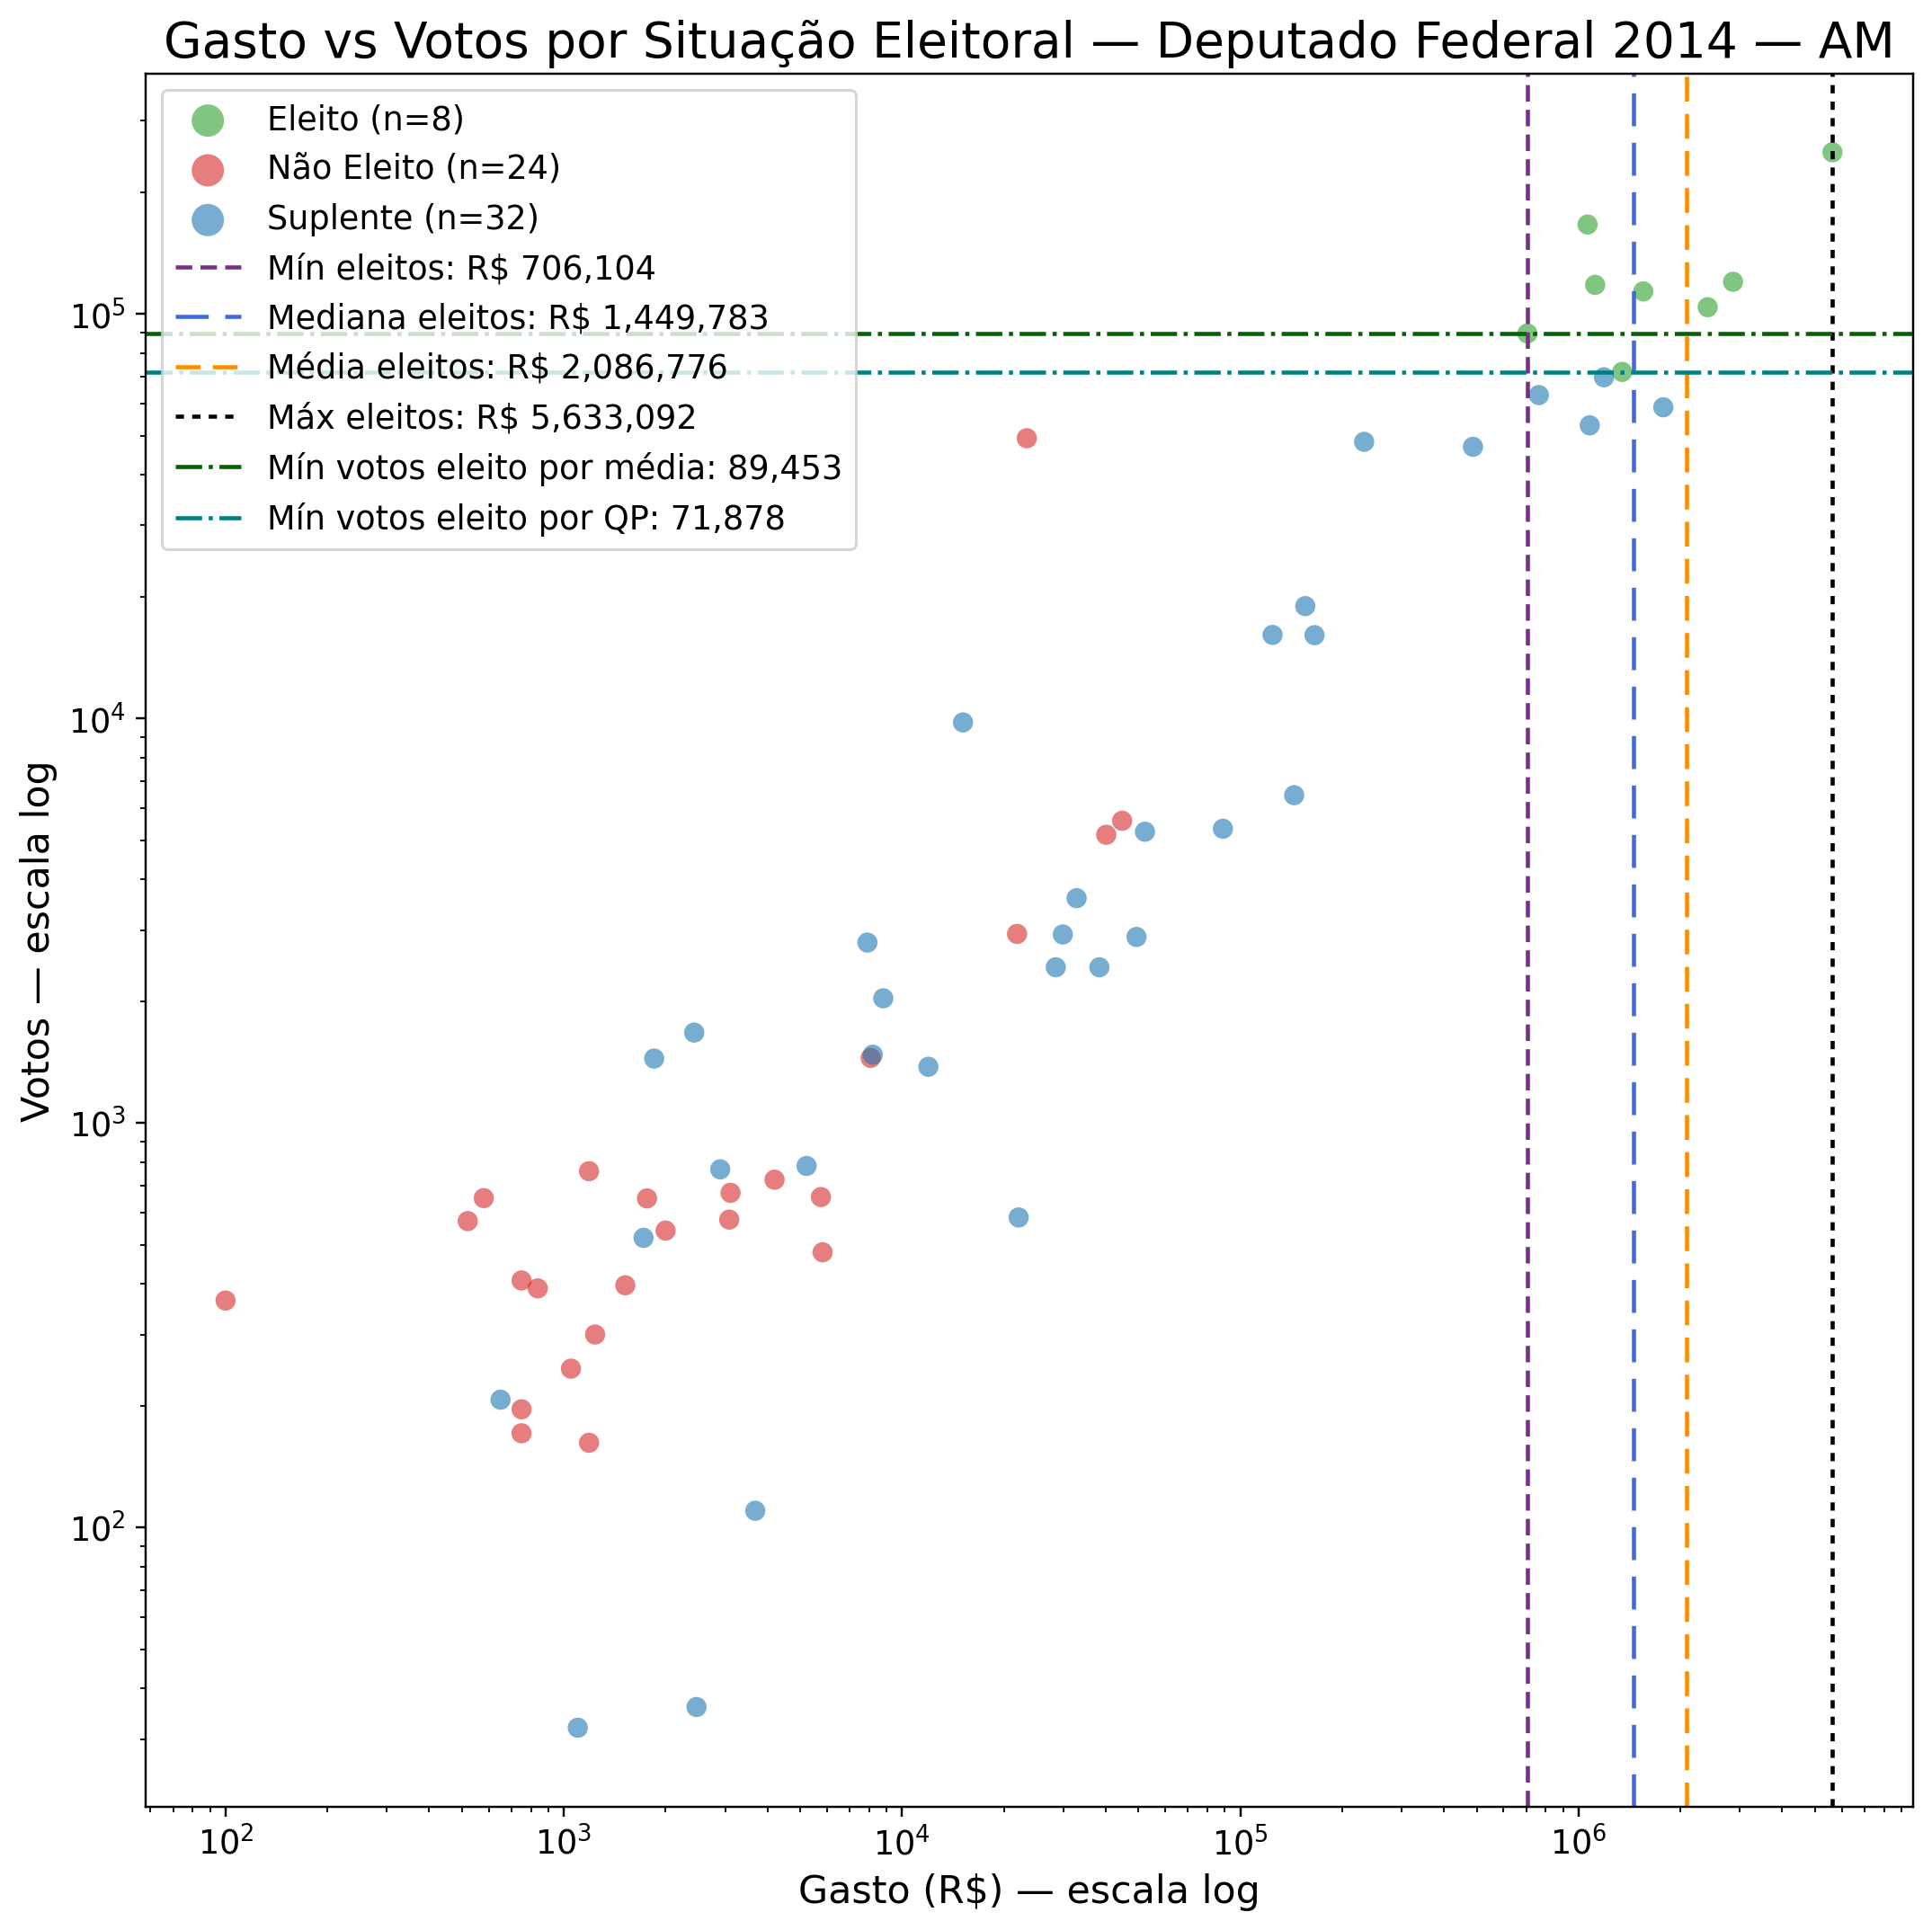
\includegraphics[width=0.98\columnwidth]{gasto_vs_votos_AM.png}
  \caption{Dispersão entre gasto e votos no Amazonas.}
  \label{fig:am_disp}
\end{figure}

No AM, o coeficiente de Pearson foi $r = 0{,}902$, a relação mais forte entre
os três estados escolhidos. A Figura~\ref{fig:am_disp} mostra uma tendência
linear muito mais nítida do que em RJ e GO, embora o menor número de
candidatos torne o resultado mais sensível a casos extremos. Ainda assim, é o
recorte em que a associação visual entre recursos e votos aparece com maior
clareza.

\subsection{Correlação por UF e Tabela-Resumo por Estado}

O briefing também exige a correlação de Pearson entre gasto e votos para todas
as UFs presentes no dataset, além de uma tabela-resumo com medidas de posição
e dispersão por estado. Esses dois resultados são apresentados nas
Tabelas~\ref{tab:corr_uf} e~\ref{tab:resumo_uf}, que devem ser inseridas a
partir dos screenshots gerados no notebook.

\begin{figure}[H]
  \centering
  \tablePlaceholder{Inserir screenshot da Tabela 3.8 do notebook.}
  \caption{Coeficiente de correlação de Pearson entre gasto e votos por UF.}
  \label{tab:corr_uf}
\end{figure}

\begin{figure}[H]
  \centering
  \tablePlaceholder{Inserir screenshot da Tabela 3.9 do notebook.}
  \caption{Tabela-resumo por UF com medidas de tendência central e dispersão
  para votos e gasto.}
  \label{tab:resumo_uf}
\end{figure}

No conjunto das UFs, a correlação foi positiva em todas as unidades presentes
na base. Os valores mais altos se concentram em estados com menos candidatos,
como AM, enquanto estados muito heterogêneos, como SP e RJ, tendem a exibir
correlações mais moderadas. Esse padrão é coerente com a ideia de que
mercados eleitorais maiores comportam mais estratégias, perfis e trajetórias
de campanha.

\subsection{Análises Extras do Notebook}

\subsubsection{Fornecedores e Setores Econômicos}

O enriquecimento com a base de fornecedores permite observar para onde o
dinheiro de campanha foi direcionado. No agregado nacional, a categoria
\texttt{\#NULO} lidera o ranking setorial, mostrando que parcela expressiva
das despesas não possui classificação econômica detalhada. Entre os setores
classificados, destacam-se organizações políticas, serviços gráficos e
comunicação visual, coerentes com a infraestrutura típica de campanhas
eleitorais em 2014.

\begin{figure}[H]
  \centering
  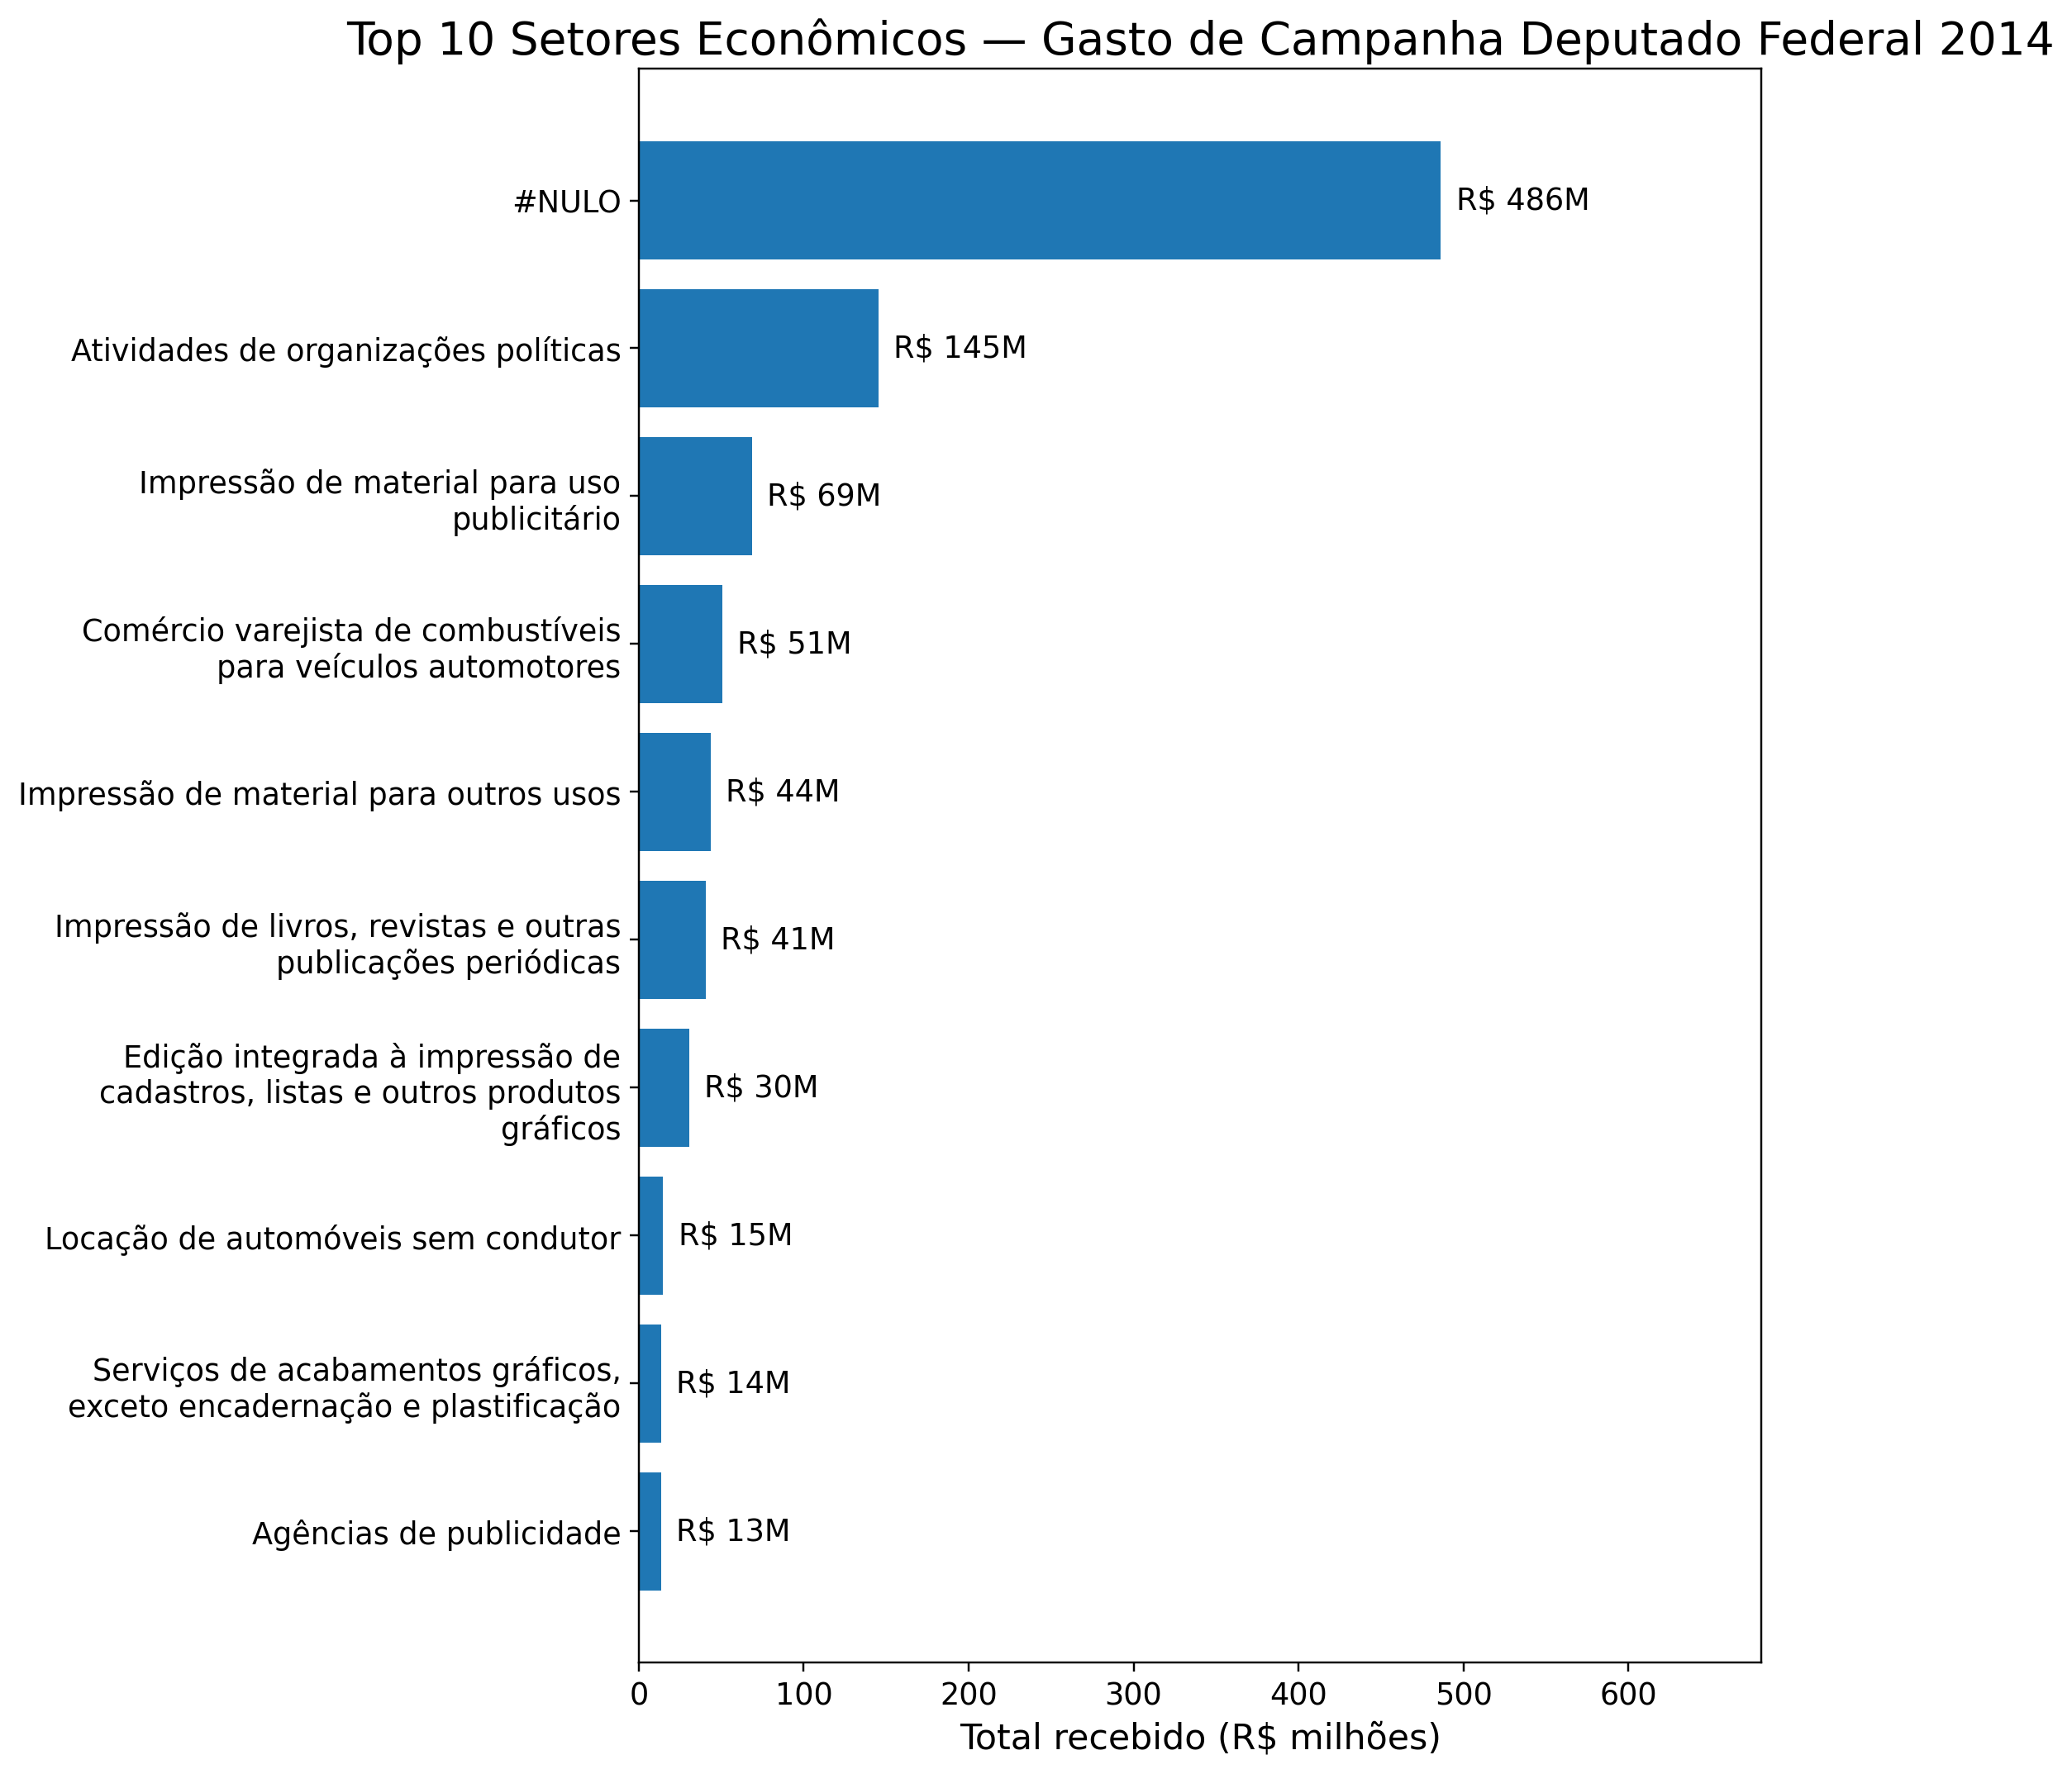
\includegraphics[width=0.98\columnwidth]{fornecedores_setores.png}
  \caption{Top 10 setores econômicos por valor recebido.}
  \label{fig:setores}
\end{figure}

A Figura~\ref{fig:setores} resume melhor a estrutura econômica das campanhas
porque mostra o padrão setorial agregado, e não apenas nomes isolados de
fornecedores. O ranking detalhado de fornecedores, gerado no notebook,
reforça essa leitura ao destacar gráficas, empresas de comunicação visual e
comitês eleitorais entre os maiores recebedores. Em termos descritivos, trata-
se de uma estrutura simultaneamente centralizada no plano partidário e
pulverizada no plano operacional.

\subsubsection{Desigualdades por Gênero e Raça}

As figuras a seguir sintetizam um dos achados mais relevantes do notebook:
o acesso aos recursos financeiros é bastante desigual entre grupos sociais,
e essa desigualdade reaparece no próprio resultado eleitoral.

\begin{figure}[H]
  \centering
  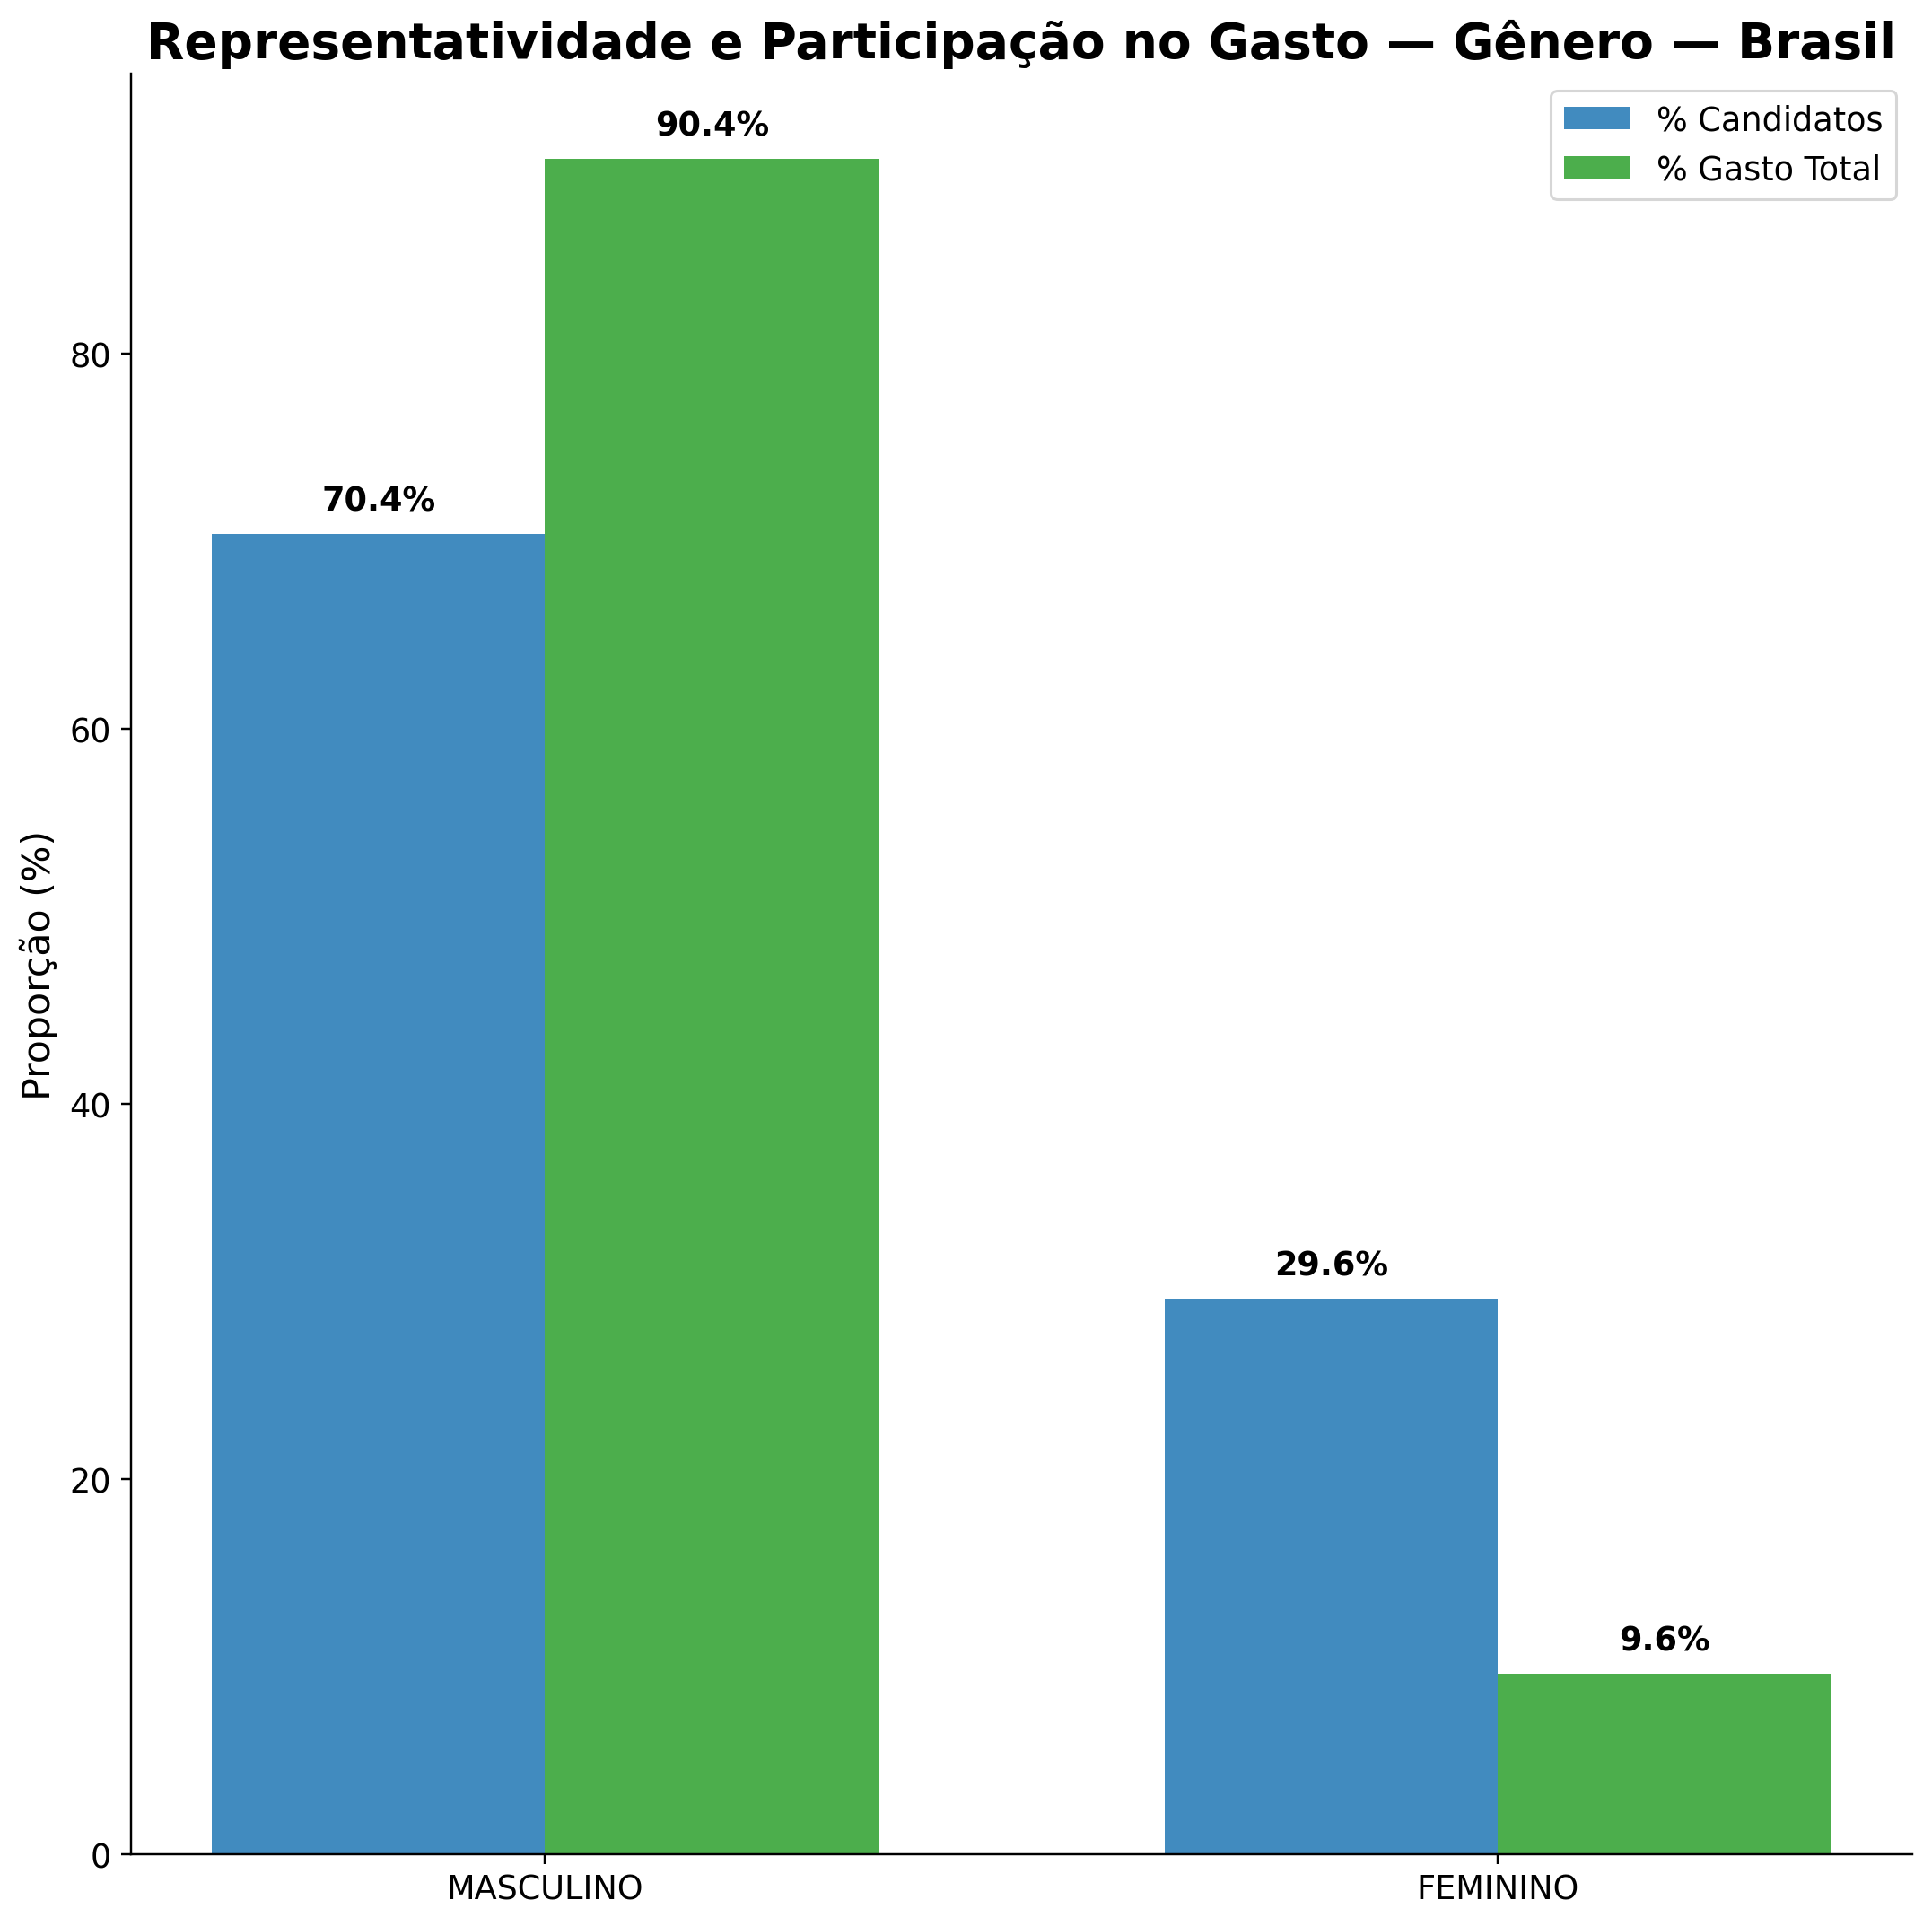
\includegraphics[width=0.98\columnwidth]{genero_representatividade.png}
  \caption{Representatividade de candidaturas e participação no gasto por gênero.}
  \label{fig:genero_representatividade}
\end{figure}

No Brasil, homens representam 70,4\% das candidaturas, mas concentram 90,4\%
do gasto total. Mulheres, por sua vez, são 29,6\% dos candidatos e acessam
apenas 9,6\% dos recursos. O gráfico deixa claro que a desigualdade não está
apenas no volume absoluto de recursos, mas na própria distribuição relativa do
financiamento entre grupos.

\begin{figure}[H]
  \centering
  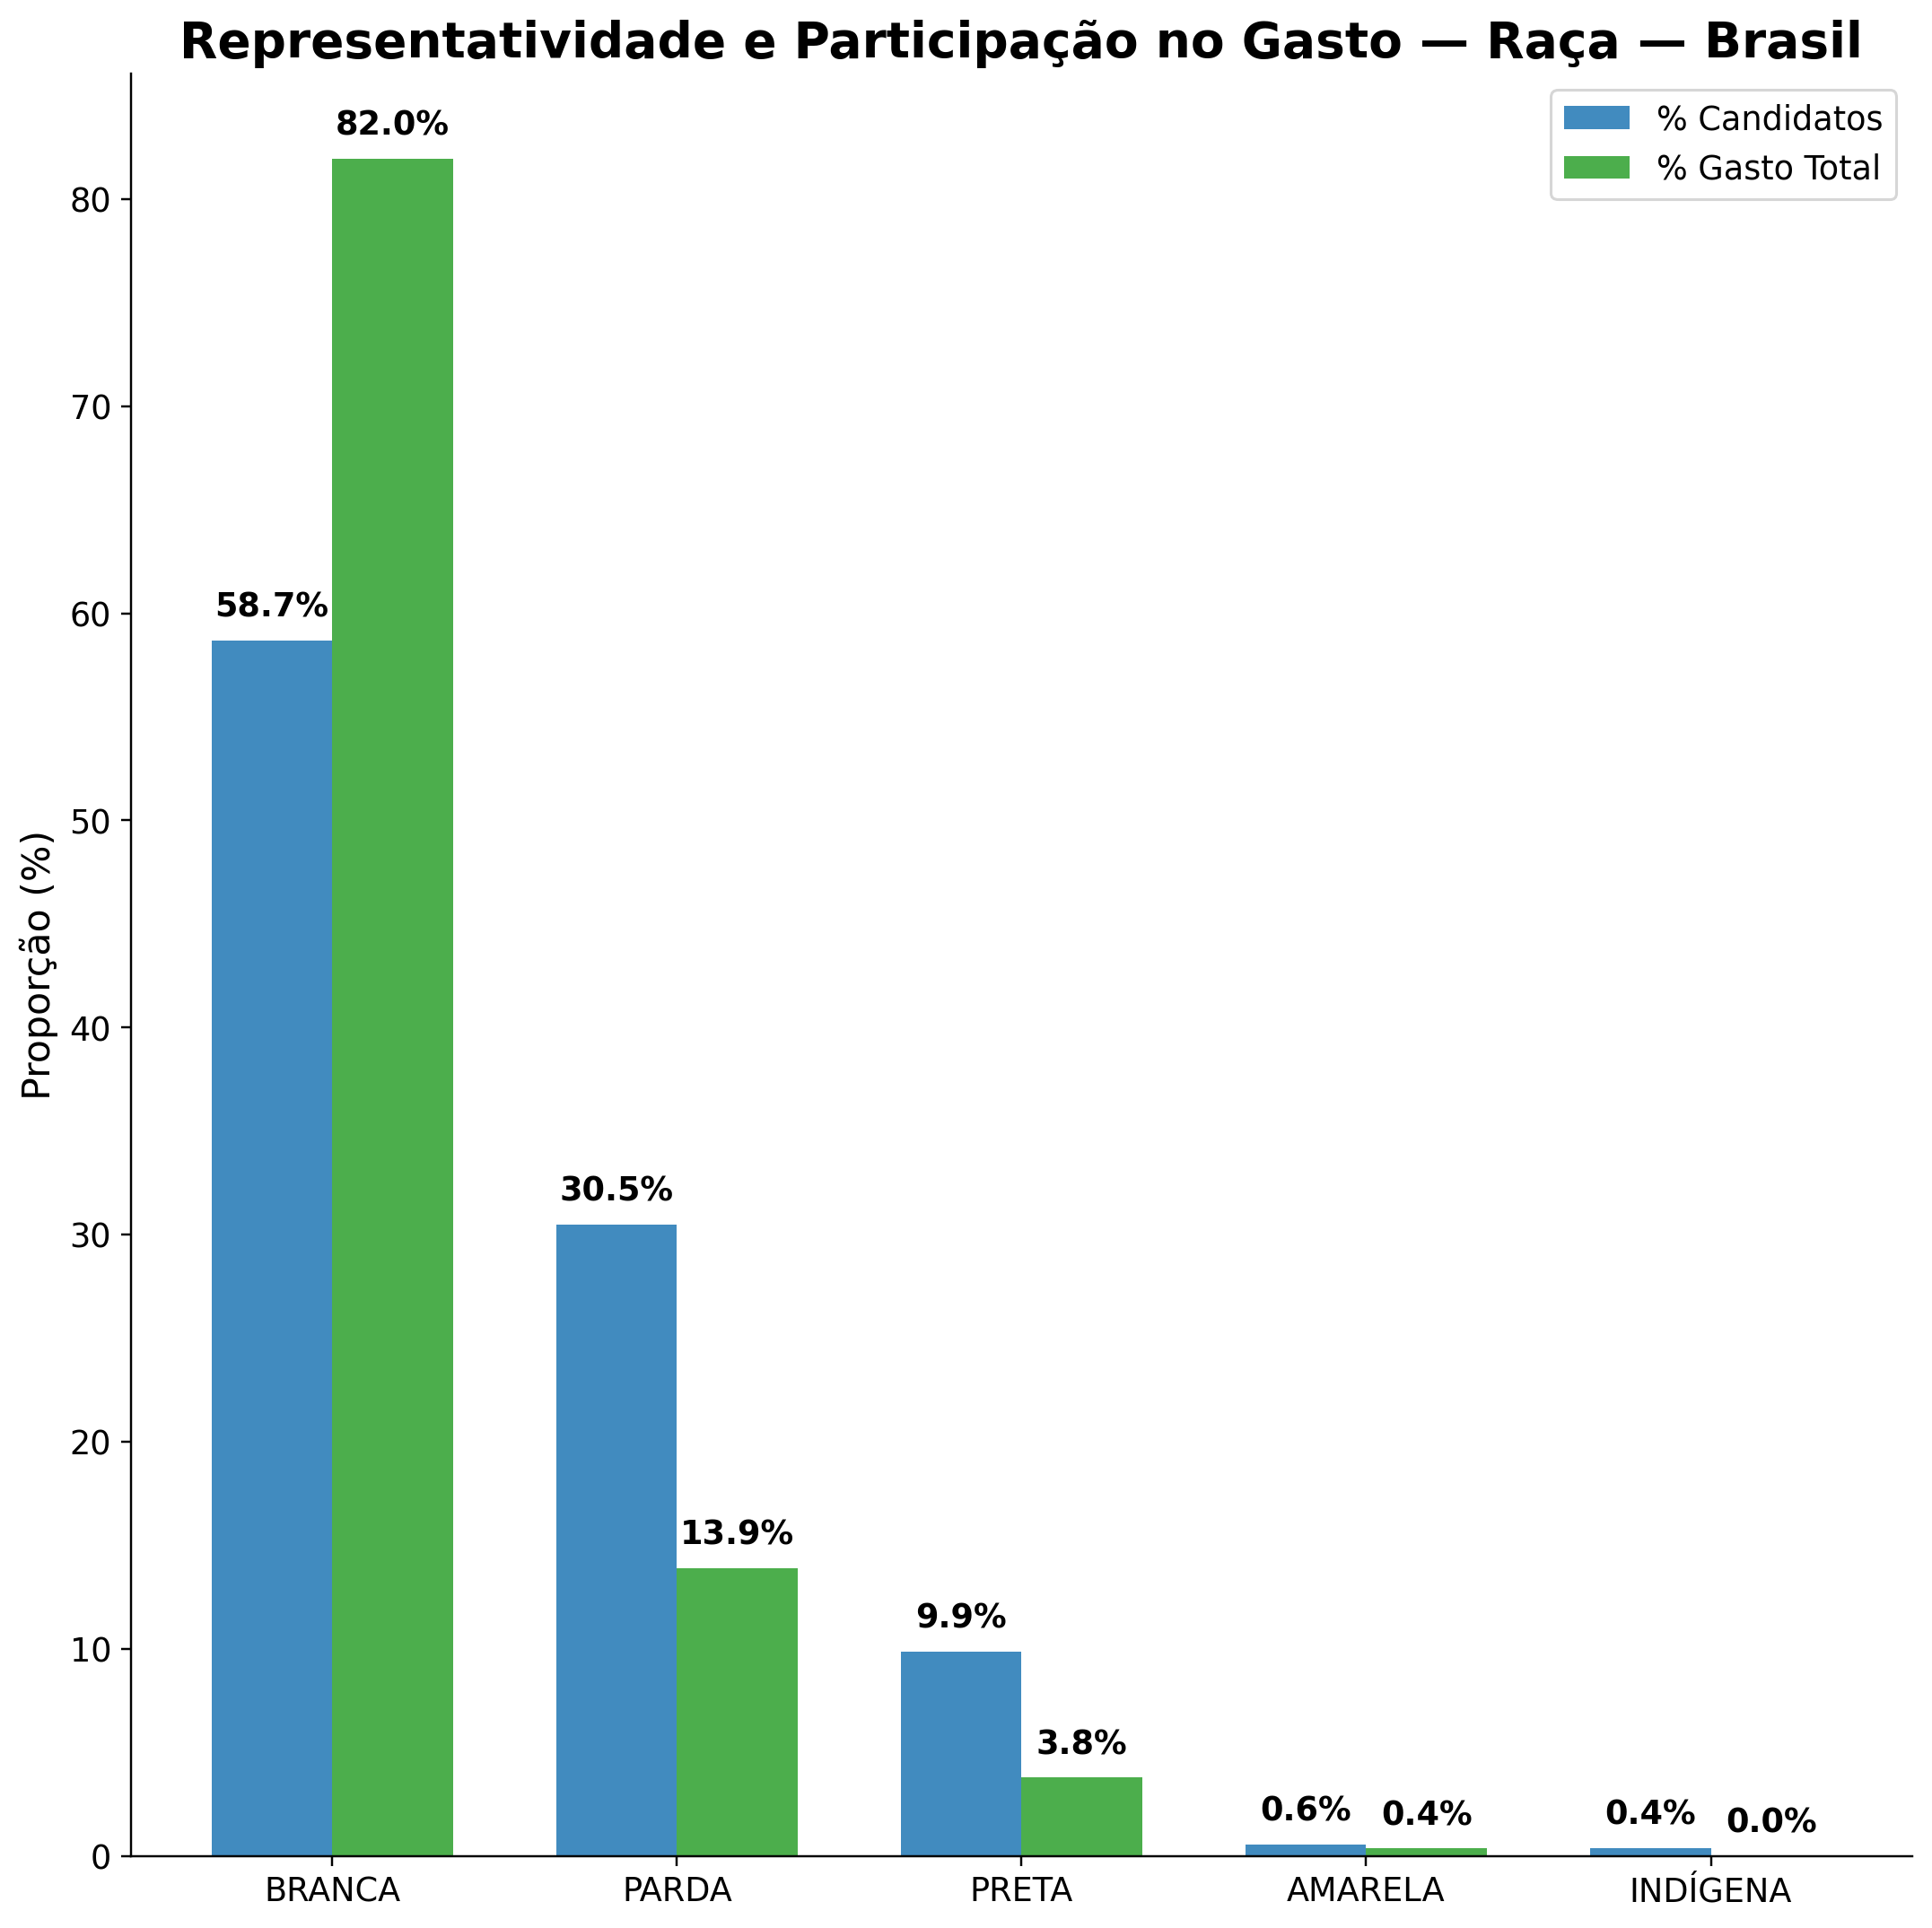
\includegraphics[width=0.98\columnwidth]{raca_representatividade.png}
  \caption{Representatividade de candidaturas e participação no gasto por raça.}
  \label{fig:raca_representatividade}
\end{figure}

Entre os grupos raciais, candidatos brancos são 58,7\% das candidaturas,
porém concentram 82,0\% do gasto, enquanto pardos e pretos ficam muito abaixo
de sua participação relativa em número de candidaturas. Esse é também o único
grupo com proporção gasto/candidatura acima de 1 no notebook, o que reforça a
interpretação de sobrerrepresentação financeira.

A desigualdade aparece também no nível individual de financiamento. No
notebook, a mediana de gasto masculino (R\$ 9.299) foi 4,6 vezes a mediana
feminina (R\$ 2.003). Entre os grupos raciais, candidatos brancos também
apresentaram as maiores medianas de gasto entre os grupos com presença
relevante na base. As visualizações de taxa de eleição, mantidas no notebook,
completam essa leitura ao mostrar que a desvantagem no acesso a recursos se
reproduz também no resultado eleitoral: mulheres e grupos raciais sub-
representados no financiamento convertem menor parcela de suas candidaturas em
cadeiras.

\FloatBarrier
\section{Conclusão}

Este artigo apresentou uma análise estatística descritiva do dataset D2 de
eleições brasileiras de 2014, cobrindo integralmente os requisitos do
briefing da disciplina e incorporando análises extras do notebook original.

Os resultados mostram que tanto gasto quanto votos possuem distribuições
fortemente assimétricas à direita, o que torna a mediana uma medida muito
mais representativa do candidato típico do que a média. A relação entre gasto
e votos foi positiva no agregado nacional e em todos os estados analisados,
com intensidades distintas: moderada em mercados eleitorais mais heterogêneos
como o RJ, moderada a forte em GO, e forte no AM.

As análises complementares revelaram ainda duas dimensões substantivas do
processo eleitoral de 2014. A primeira é a importância de estruturas
intermediárias de campanha, como comitês partidários e fornecedores gráficos,
na circulação dos recursos. A segunda é a persistência de desigualdades no
acesso ao financiamento: homens e candidatos brancos concentram parcela dos
recursos superior ao seu peso nas candidaturas, enquanto mulheres, pardos,
pretos e indígenas aparecem subfinanciados.

Em síntese, o dataset confirma que recursos financeiros estão associados ao
desempenho eleitoral, mas também sugere que o acesso desigual a esses
recursos pode funcionar como barreira estrutural à competição política de
grupos sub-representados.

\end{document}
